% Options for packages loaded elsewhere
% Options for packages loaded elsewhere
\PassOptionsToPackage{unicode}{hyperref}
\PassOptionsToPackage{hyphens}{url}
\PassOptionsToPackage{dvipsnames,svgnames,x11names}{xcolor}
%
\documentclass[
  letterpaper,
  DIV=11,
  numbers=noendperiod]{scrartcl}
\usepackage{xcolor}
\usepackage{amsmath,amssymb}
\setcounter{secnumdepth}{5}
\usepackage{iftex}
\ifPDFTeX
  \usepackage[T1]{fontenc}
  \usepackage[utf8]{inputenc}
  \usepackage{textcomp} % provide euro and other symbols
\else % if luatex or xetex
  \usepackage{unicode-math} % this also loads fontspec
  \defaultfontfeatures{Scale=MatchLowercase}
  \defaultfontfeatures[\rmfamily]{Ligatures=TeX,Scale=1}
\fi
\usepackage{lmodern}
\ifPDFTeX\else
  % xetex/luatex font selection
\fi
% Use upquote if available, for straight quotes in verbatim environments
\IfFileExists{upquote.sty}{\usepackage{upquote}}{}
\IfFileExists{microtype.sty}{% use microtype if available
  \usepackage[]{microtype}
  \UseMicrotypeSet[protrusion]{basicmath} % disable protrusion for tt fonts
}{}
\makeatletter
\@ifundefined{KOMAClassName}{% if non-KOMA class
  \IfFileExists{parskip.sty}{%
    \usepackage{parskip}
  }{% else
    \setlength{\parindent}{0pt}
    \setlength{\parskip}{6pt plus 2pt minus 1pt}}
}{% if KOMA class
  \KOMAoptions{parskip=half}}
\makeatother
% Make \paragraph and \subparagraph free-standing
\makeatletter
\ifx\paragraph\undefined\else
  \let\oldparagraph\paragraph
  \renewcommand{\paragraph}{
    \@ifstar
      \xxxParagraphStar
      \xxxParagraphNoStar
  }
  \newcommand{\xxxParagraphStar}[1]{\oldparagraph*{#1}\mbox{}}
  \newcommand{\xxxParagraphNoStar}[1]{\oldparagraph{#1}\mbox{}}
\fi
\ifx\subparagraph\undefined\else
  \let\oldsubparagraph\subparagraph
  \renewcommand{\subparagraph}{
    \@ifstar
      \xxxSubParagraphStar
      \xxxSubParagraphNoStar
  }
  \newcommand{\xxxSubParagraphStar}[1]{\oldsubparagraph*{#1}\mbox{}}
  \newcommand{\xxxSubParagraphNoStar}[1]{\oldsubparagraph{#1}\mbox{}}
\fi
\makeatother


\usepackage{longtable,booktabs,array}
\usepackage{calc} % for calculating minipage widths
% Correct order of tables after \paragraph or \subparagraph
\usepackage{etoolbox}
\makeatletter
\patchcmd\longtable{\par}{\if@noskipsec\mbox{}\fi\par}{}{}
\makeatother
% Allow footnotes in longtable head/foot
\IfFileExists{footnotehyper.sty}{\usepackage{footnotehyper}}{\usepackage{footnote}}
\makesavenoteenv{longtable}
\usepackage{graphicx}
\makeatletter
\newsavebox\pandoc@box
\newcommand*\pandocbounded[1]{% scales image to fit in text height/width
  \sbox\pandoc@box{#1}%
  \Gscale@div\@tempa{\textheight}{\dimexpr\ht\pandoc@box+\dp\pandoc@box\relax}%
  \Gscale@div\@tempb{\linewidth}{\wd\pandoc@box}%
  \ifdim\@tempb\p@<\@tempa\p@\let\@tempa\@tempb\fi% select the smaller of both
  \ifdim\@tempa\p@<\p@\scalebox{\@tempa}{\usebox\pandoc@box}%
  \else\usebox{\pandoc@box}%
  \fi%
}
% Set default figure placement to htbp
\def\fps@figure{htbp}
\makeatother





\setlength{\emergencystretch}{3em} % prevent overfull lines

\providecommand{\tightlist}{%
  \setlength{\itemsep}{0pt}\setlength{\parskip}{0pt}}



 


\KOMAoption{captions}{tableheading}
\makeatletter
\@ifpackageloaded{caption}{}{\usepackage{caption}}
\AtBeginDocument{%
\ifdefined\contentsname
  \renewcommand*\contentsname{Table of contents}
\else
  \newcommand\contentsname{Table of contents}
\fi
\ifdefined\listfigurename
  \renewcommand*\listfigurename{List of Figures}
\else
  \newcommand\listfigurename{List of Figures}
\fi
\ifdefined\listtablename
  \renewcommand*\listtablename{List of Tables}
\else
  \newcommand\listtablename{List of Tables}
\fi
\ifdefined\figurename
  \renewcommand*\figurename{Figure}
\else
  \newcommand\figurename{Figure}
\fi
\ifdefined\tablename
  \renewcommand*\tablename{Table}
\else
  \newcommand\tablename{Table}
\fi
}
\@ifpackageloaded{float}{}{\usepackage{float}}
\floatstyle{ruled}
\@ifundefined{c@chapter}{\newfloat{codelisting}{h}{lop}}{\newfloat{codelisting}{h}{lop}[chapter]}
\floatname{codelisting}{Listing}
\newcommand*\listoflistings{\listof{codelisting}{List of Listings}}
\makeatother
\makeatletter
\makeatother
\makeatletter
\@ifpackageloaded{caption}{}{\usepackage{caption}}
\@ifpackageloaded{subcaption}{}{\usepackage{subcaption}}
\makeatother
\usepackage{bookmark}
\IfFileExists{xurl.sty}{\usepackage{xurl}}{} % add URL line breaks if available
\urlstyle{same}
\hypersetup{
  pdftitle={Inflation Analysis Report},
  colorlinks=true,
  linkcolor={blue},
  filecolor={Maroon},
  citecolor={Blue},
  urlcolor={Blue},
  pdfcreator={LaTeX via pandoc}}


\title{Inflation Analysis Report}
\author{}
\date{2026-01-12}
\begin{document}
\maketitle

\renewcommand*\contentsname{Table of contents}
{
\hypersetup{linkcolor=}
\setcounter{tocdepth}{3}
\tableofcontents
}

\section{Overall Consumer Price Index
Heatmap}\label{overall-consumer-price-index-heatmap}

\subsection{Year-on-Year Change}\label{year-on-year-change}

\begin{figure}[H]

\centering{

\pandocbounded{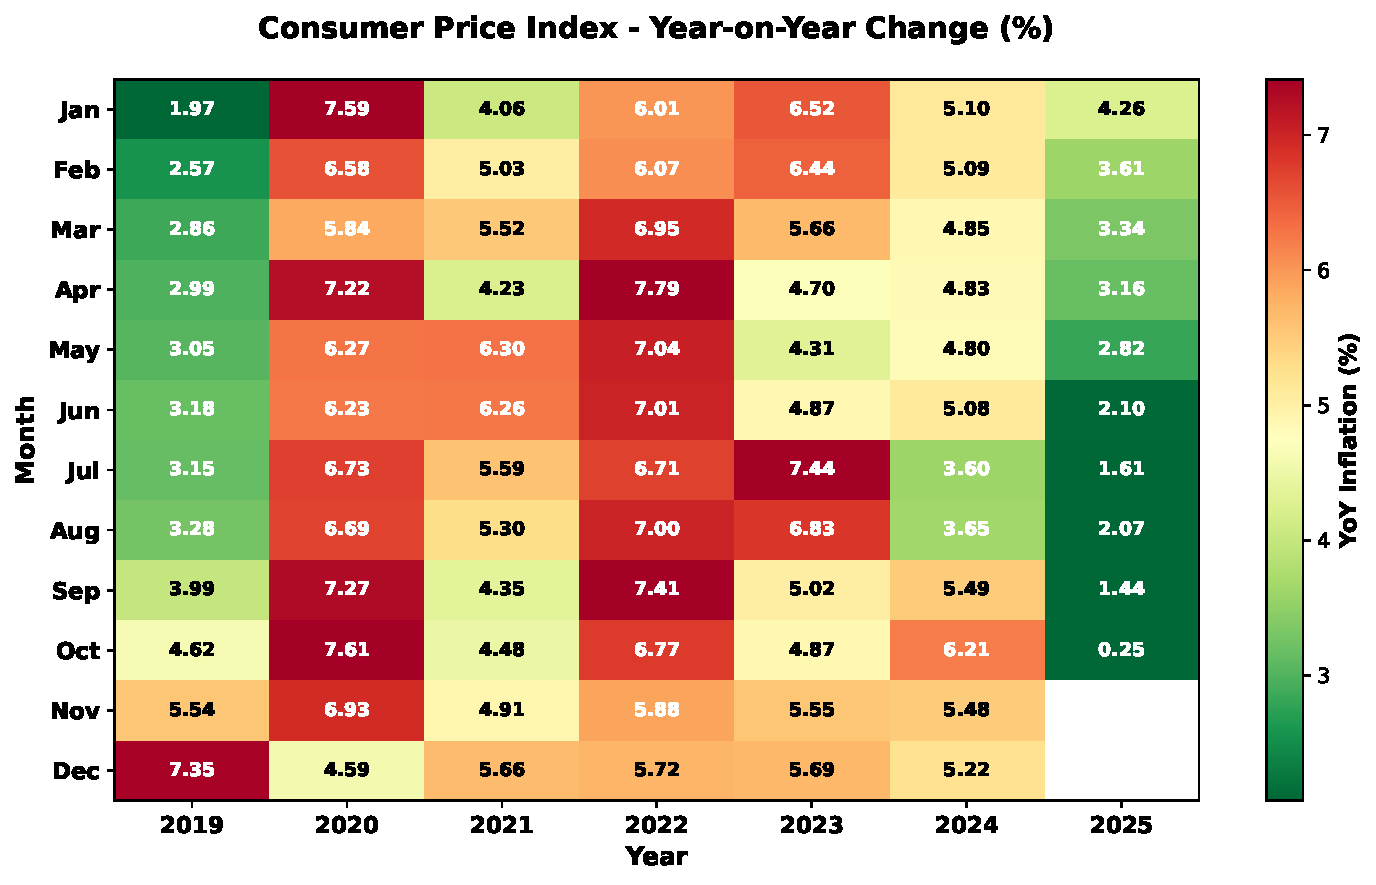
\includegraphics[keepaspectratio]{inflation_analysis_files/figure-pdf/fig-yoy-heatmap-output-1.pdf}}

}

\caption{\label{fig-yoy-heatmap}Consumer Price Index - Year-on-Year
Change Heatmap}

\end{figure}%

\subsection{Month-on-Month Change}\label{month-on-month-change}

\begin{figure}[H]

\centering{

\pandocbounded{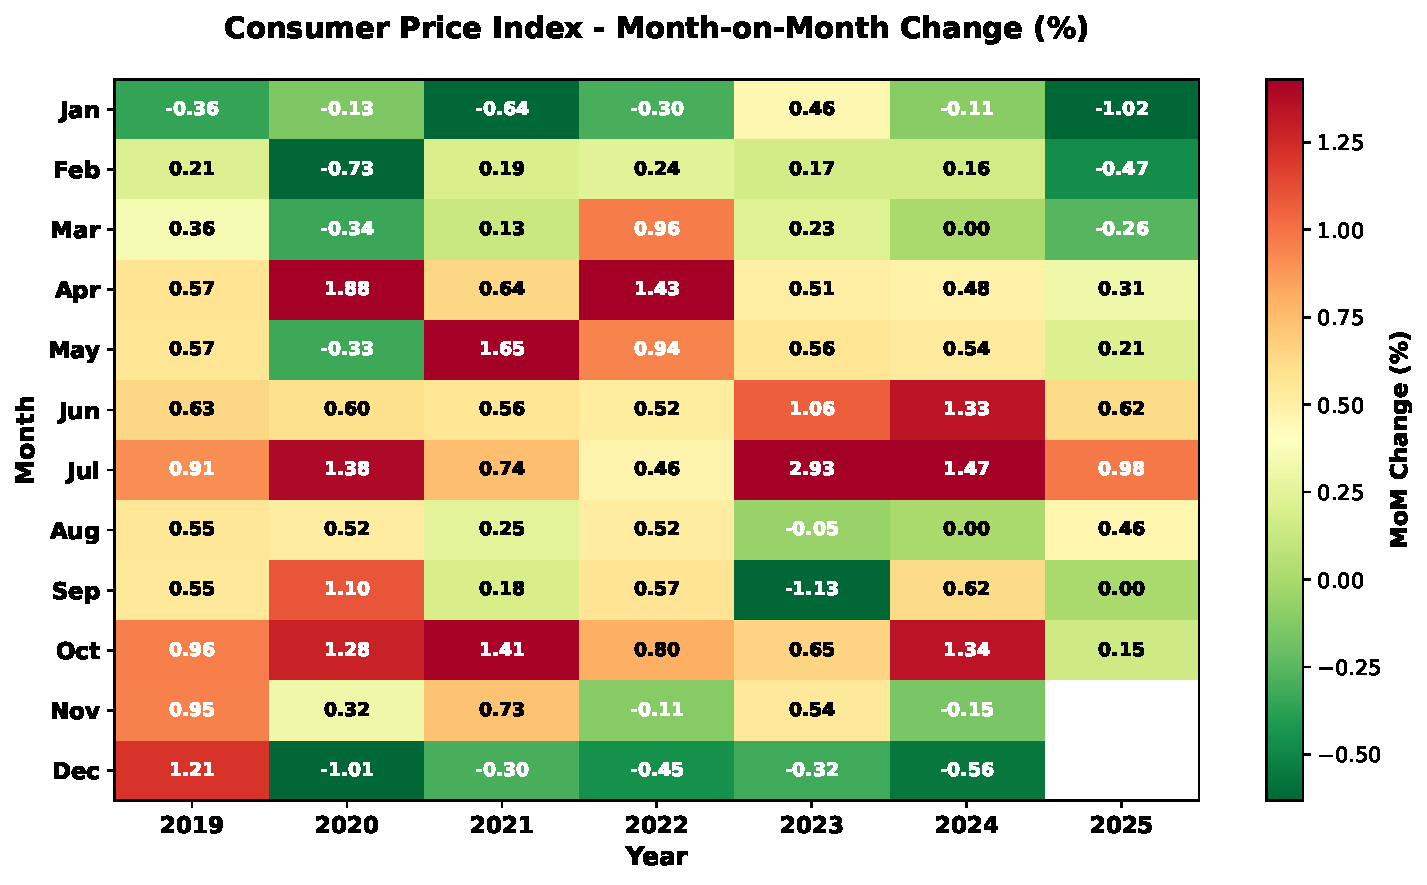
\includegraphics[keepaspectratio]{inflation_analysis_files/figure-pdf/fig-mom-heatmap-output-1.pdf}}

}

\caption{\label{fig-mom-heatmap}Consumer Price Index - Month-on-Month
Change Heatmap}

\end{figure}%

\section{Top 5 Changes}\label{top-5-changes}

\begin{figure}[H]

\centering{

\pandocbounded{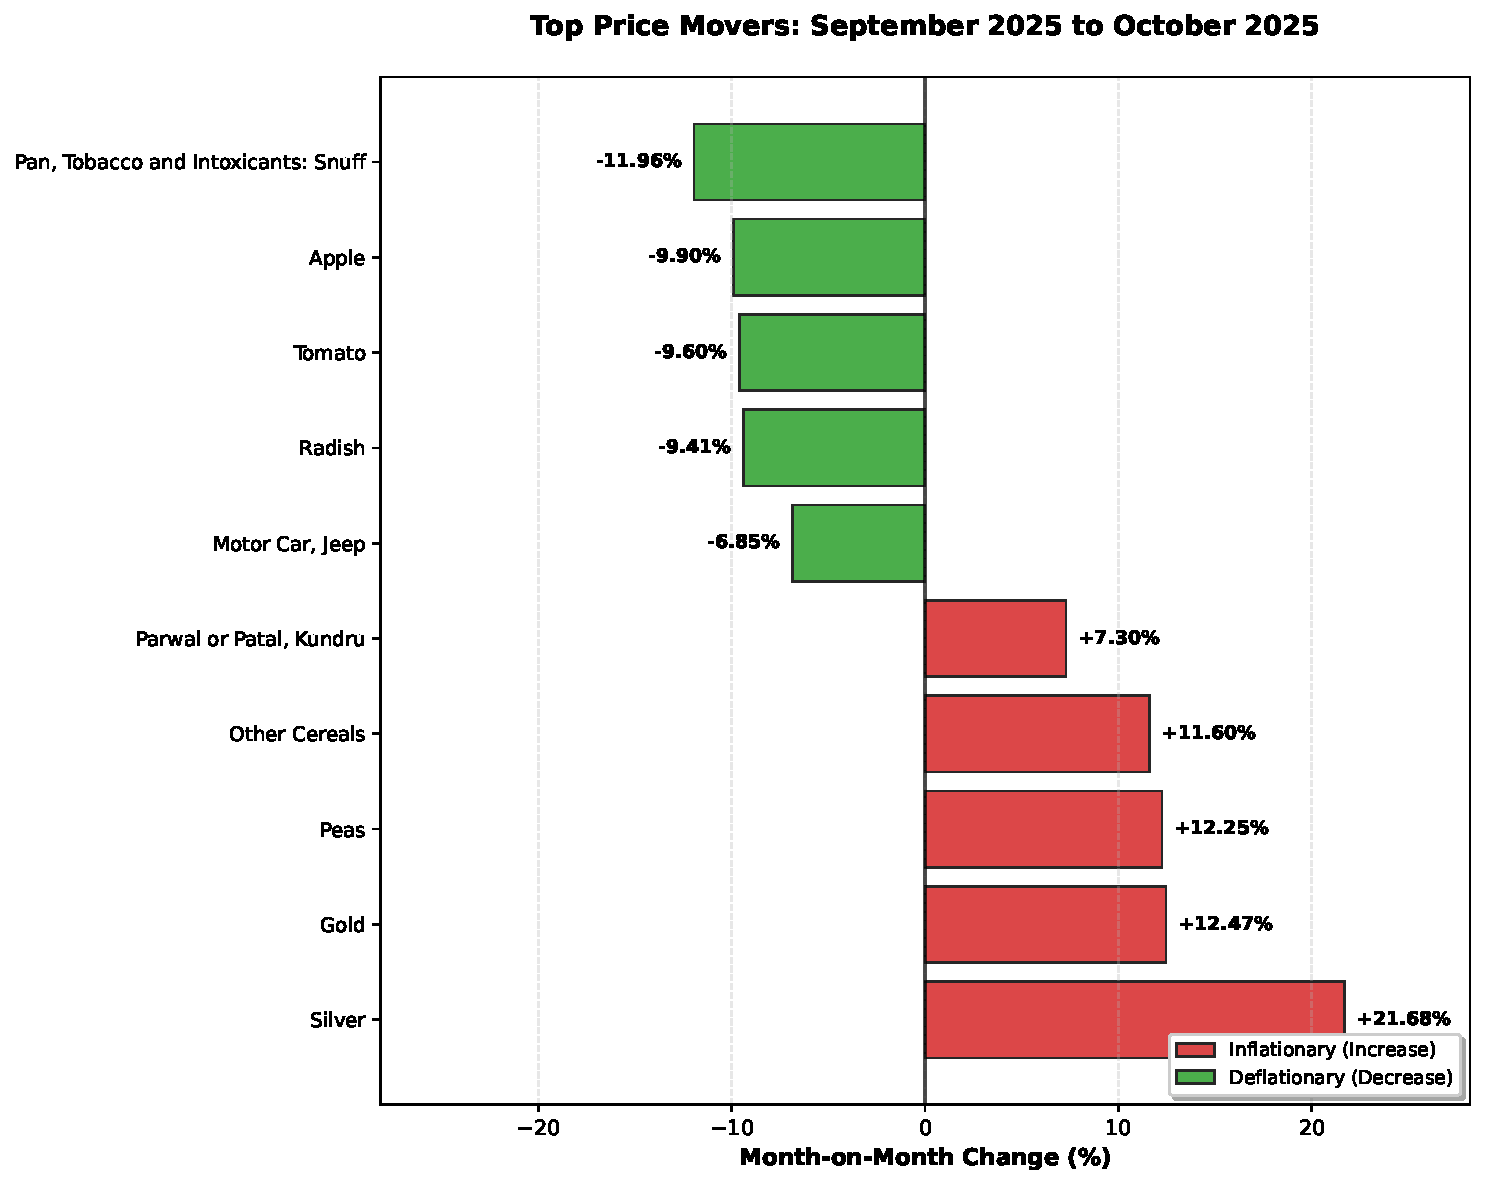
\includegraphics[keepaspectratio]{inflation_analysis_files/figure-pdf/fig-top-changes-output-1.pdf}}

}

\caption{\label{fig-top-changes}Top Inflationary and Deflationary
Categories (Month-on-Month)}

\end{figure}%

\subsection{Key Observations}\label{key-observations}

\begin{itemize}
\item
  \textbf{Silver} experienced the highest inflationary pressure with a
  \textbf{21.68\%} increase.
\item
  \textbf{Motor Car, Jeep} showed the largest deflationary trend with a
  \textbf{-6.85\%} decrease.
\end{itemize}

\subsection{Year-on-Year Top Movers}\label{year-on-year-top-movers}

\begin{figure}[H]

\centering{

\pandocbounded{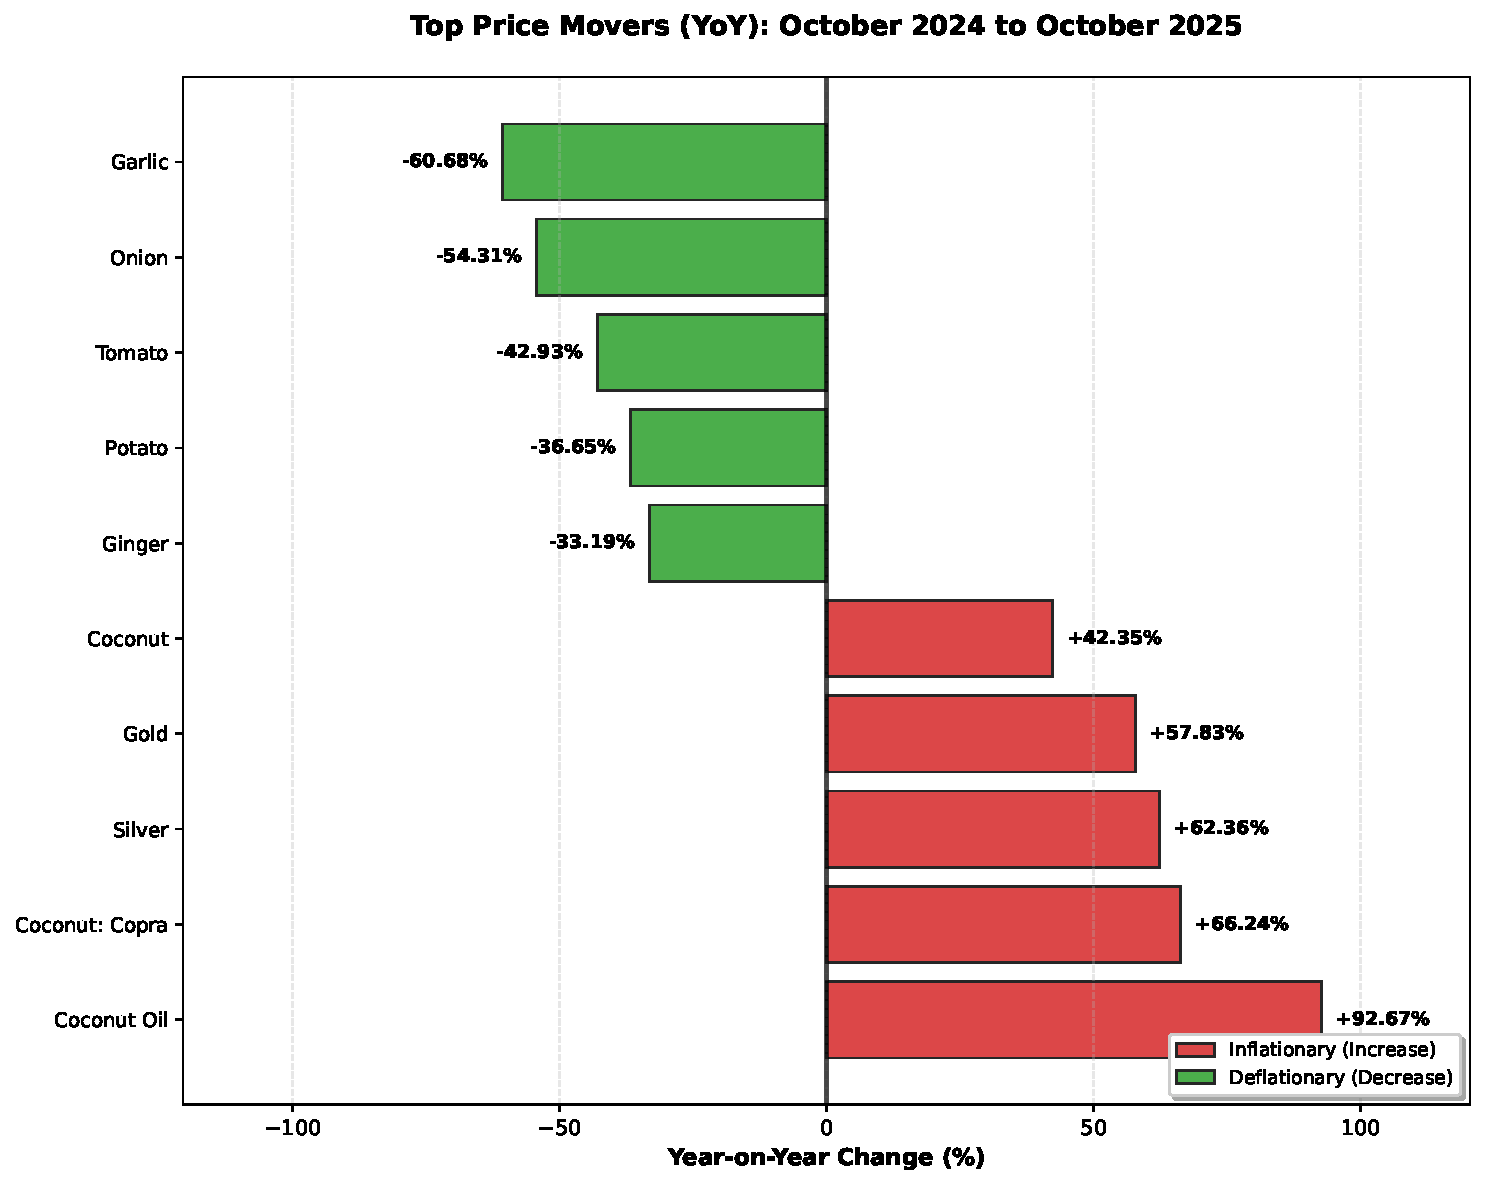
\includegraphics[keepaspectratio]{inflation_analysis_files/figure-pdf/fig-top-changes-yoy-output-1.pdf}}

}

\caption{\label{fig-top-changes-yoy}Top Inflationary and Deflationary
Categories (Year-on-Year)}

\end{figure}%

\subsubsection{Key Observations (YoY)}\label{key-observations-yoy}

\begin{itemize}
\item
  \textbf{Coconut Oil} experienced the highest year-on-year inflationary
  pressure with a \textbf{92.67\%} increase.
\item
  \textbf{Ginger} showed the largest year-on-year deflationary trend
  with a \textbf{-33.19\%} decrease.
\end{itemize}

\section{Inflation Dispersion
Analysis}\label{inflation-dispersion-analysis}

This section analyzes how inflation is distributed across different CPI
components, showing whether price changes are broad-based or
concentrated in specific items.

\subsection{Distribution Over Time
(Normalized)}\label{distribution-over-time-normalized}

\begin{figure}[H]

\centering{

\pandocbounded{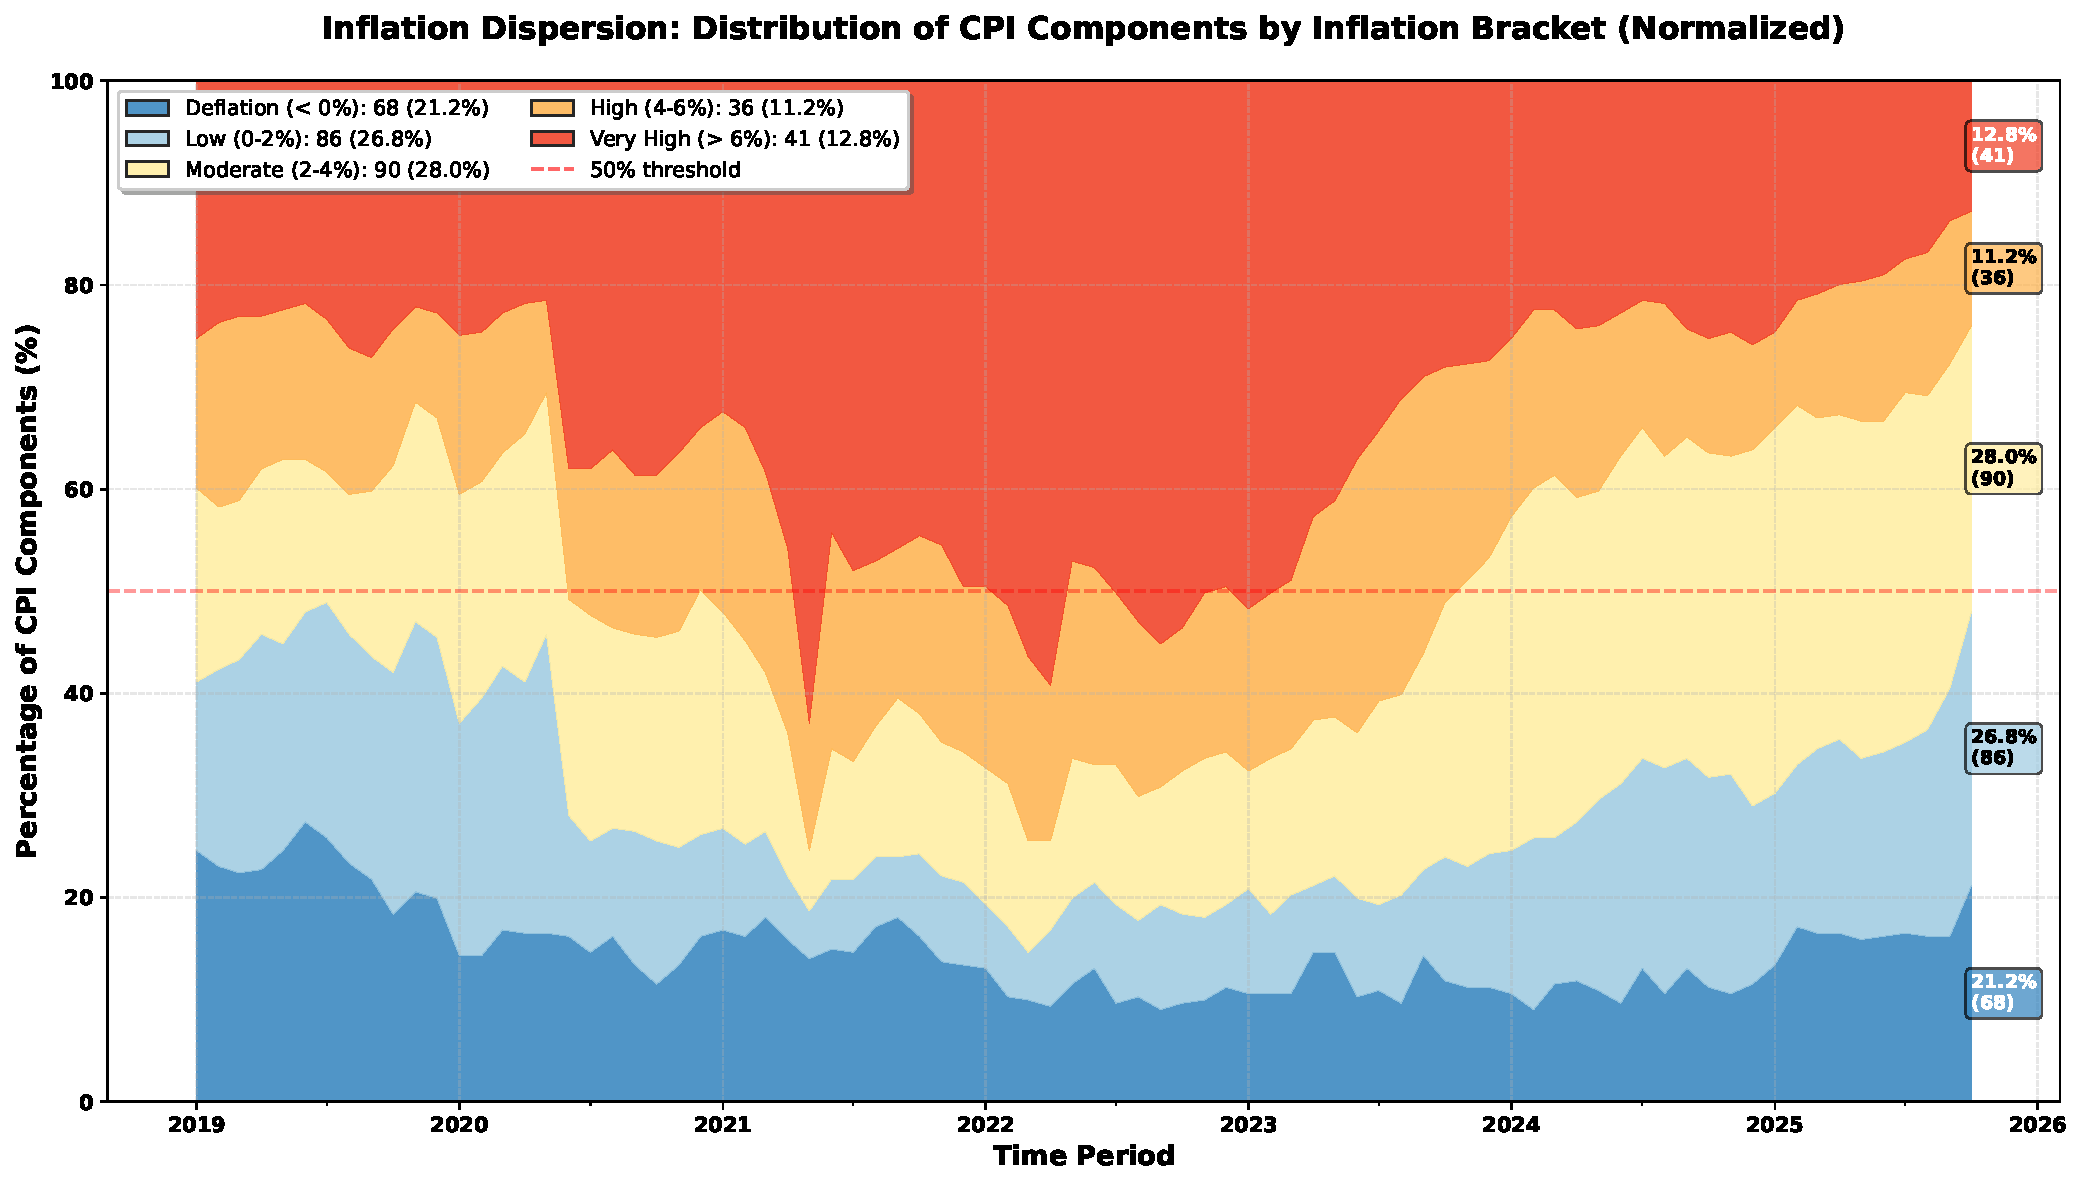
\includegraphics[keepaspectratio]{inflation_analysis_files/figure-pdf/fig-dispersion-normalized-output-1.pdf}}

}

\caption{\label{fig-dispersion-normalized}Inflation Dispersion -
Percentage of CPI Components by Bracket}

\end{figure}%

\subsection{Recent Trends (Last 3
Years)}\label{recent-trends-last-3-years}

\begin{figure}[H]

\centering{

\pandocbounded{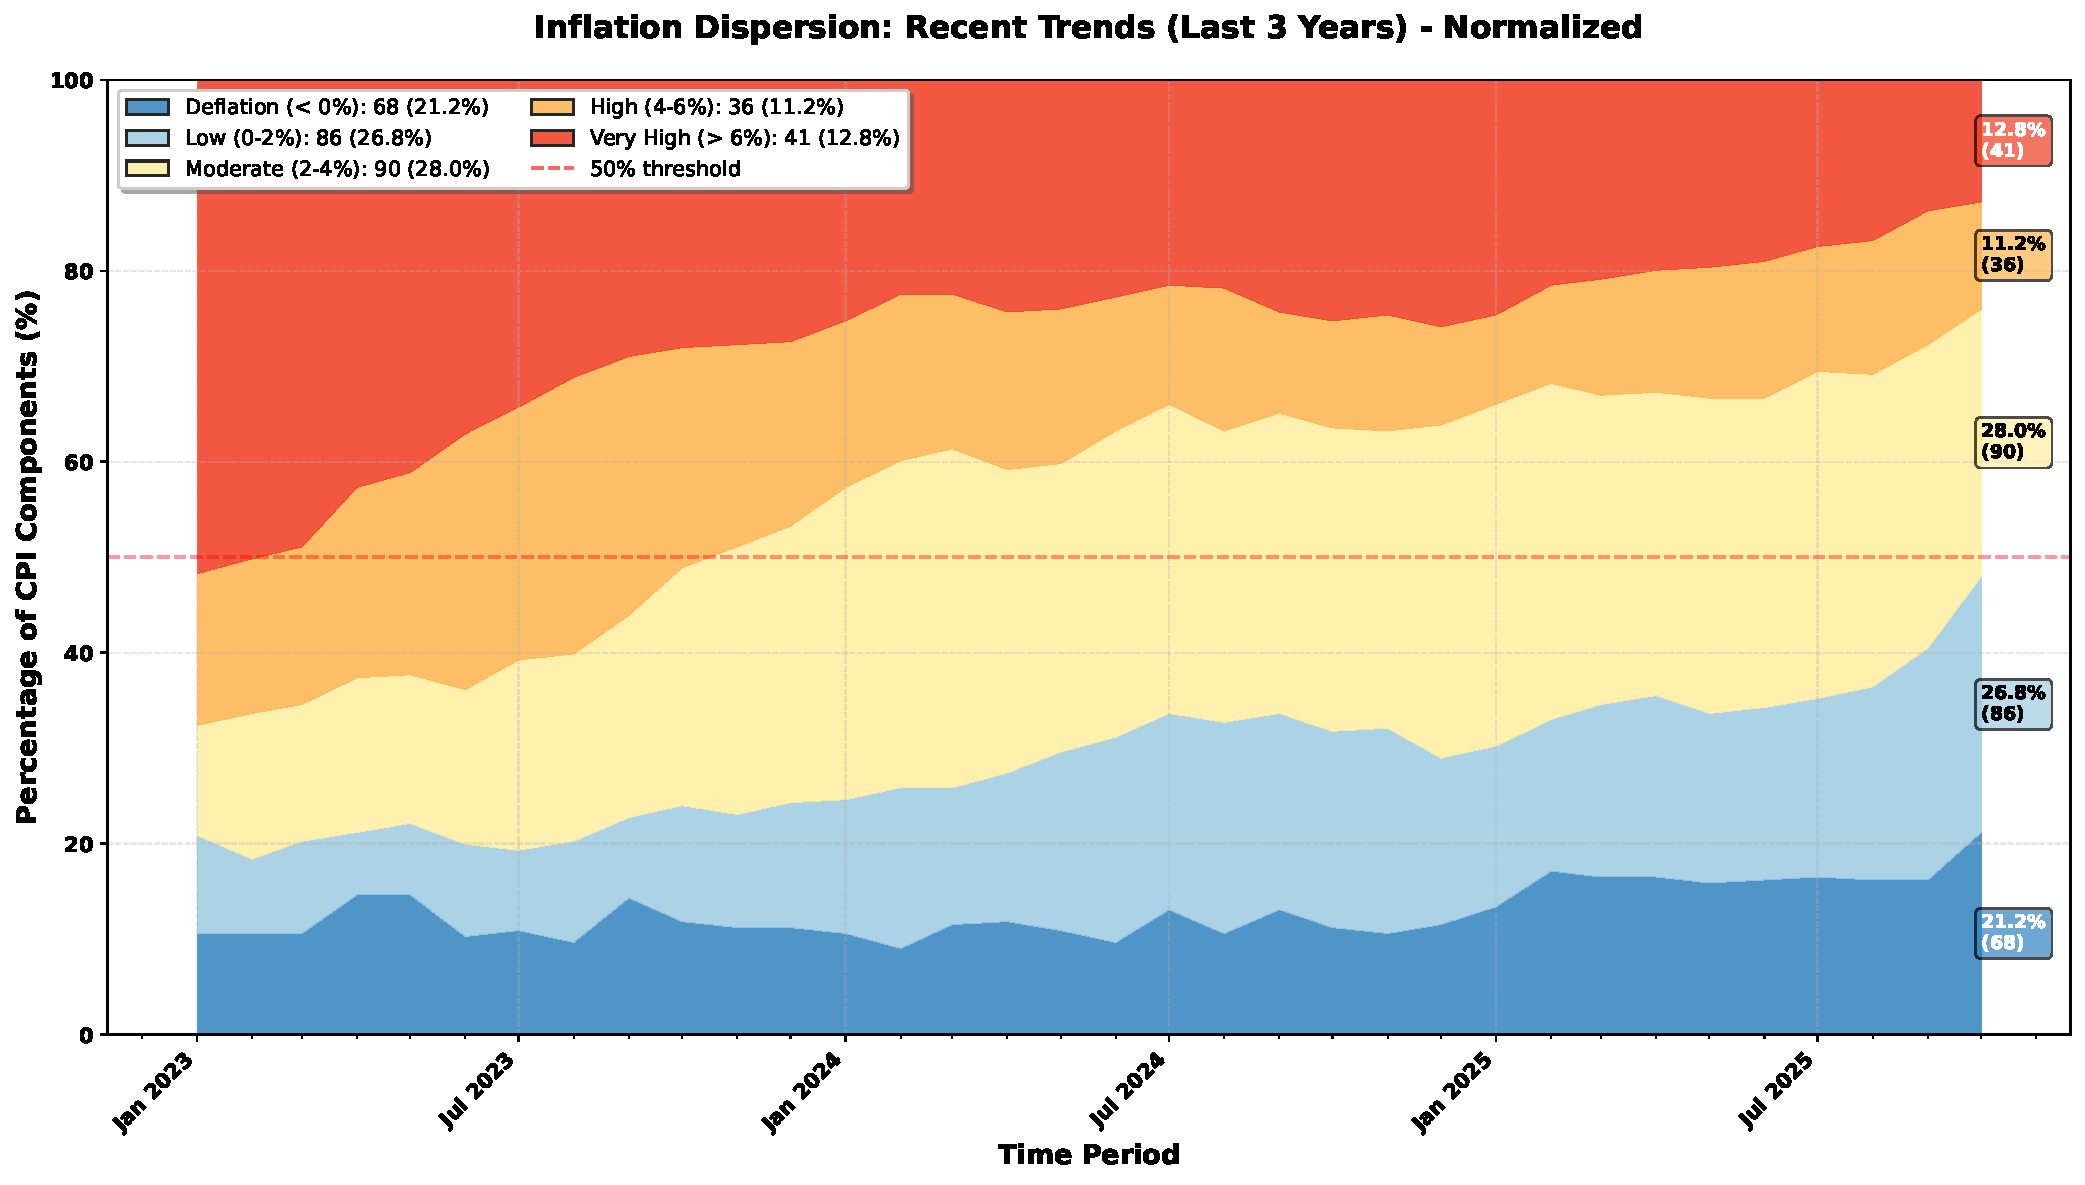
\includegraphics[keepaspectratio]{inflation_analysis_files/figure-pdf/fig-dispersion-normalized-3yr-output-1.pdf}}

}

\caption{\label{fig-dispersion-normalized-3yr}Inflation Dispersion -
Last 3 Years (Normalized)}

\end{figure}%

\subsection{Distribution Over Time (Absolute
Counts)}\label{distribution-over-time-absolute-counts}

\begin{figure}[H]

\centering{

\pandocbounded{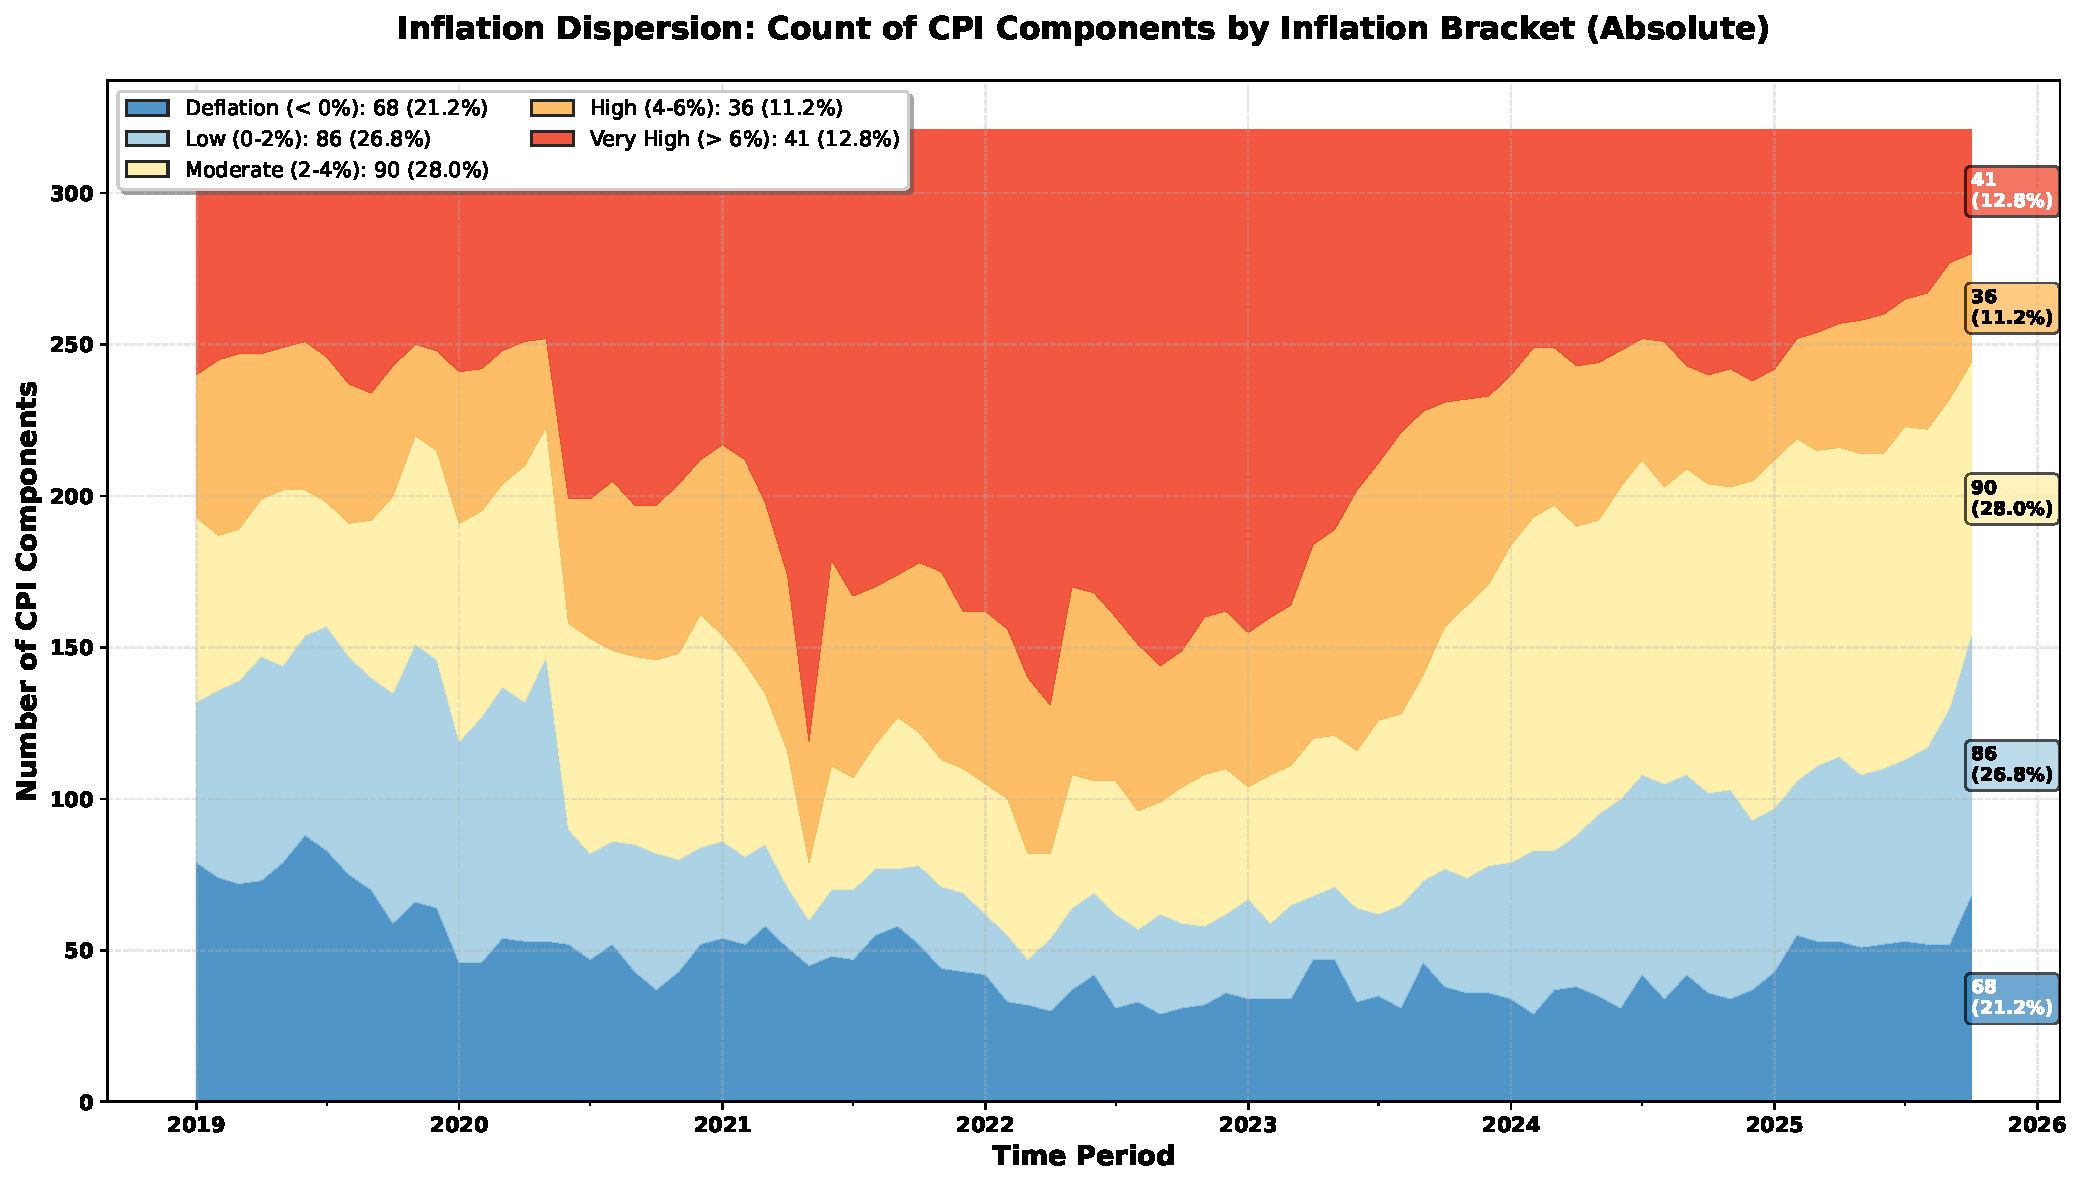
\includegraphics[keepaspectratio]{inflation_analysis_files/figure-pdf/fig-dispersion-absolute-output-1.pdf}}

}

\caption{\label{fig-dispersion-absolute}Inflation Dispersion - Absolute
Count of CPI Components by Bracket}

\end{figure}%

\subsection{Recent Trends (Last 3 Years -
Absolute)}\label{recent-trends-last-3-years---absolute}

\begin{figure}[H]

\centering{

\pandocbounded{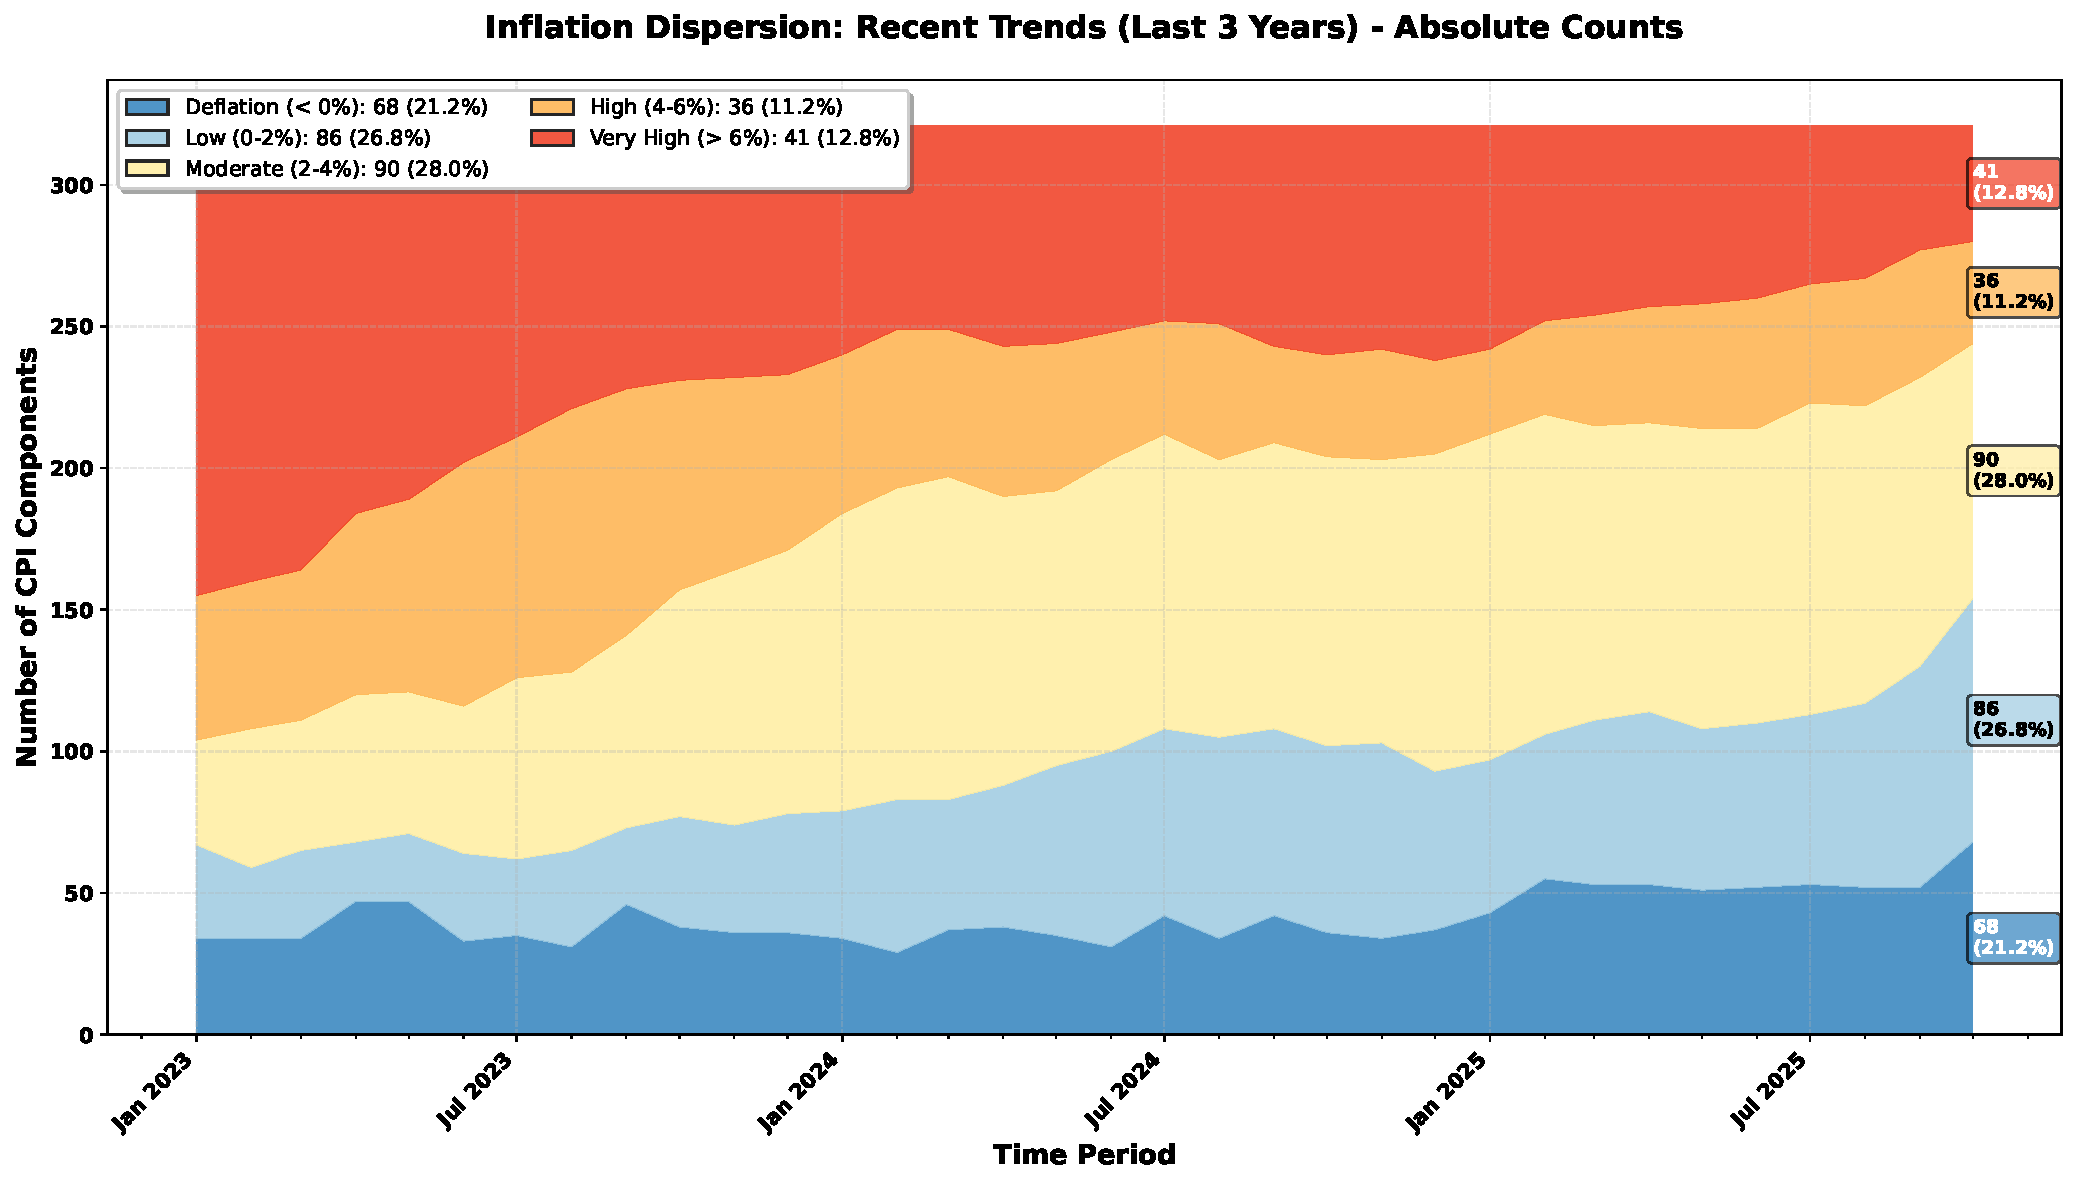
\includegraphics[keepaspectratio]{inflation_analysis_files/figure-pdf/fig-dispersion-absolute-3yr-output-1.pdf}}

}

\caption{\label{fig-dispersion-absolute-3yr}Inflation Dispersion - Last
3 Years (Absolute Counts)}

\end{figure}%

\subsection{Annualized MoM Threshold
Analysis}\label{annualized-mom-threshold-analysis}

\subsubsection{6\% Annualized Threshold (0.5\%
MoM)}\label{annualized-threshold-0.5-mom}

\begin{figure}[H]

\centering{

\pandocbounded{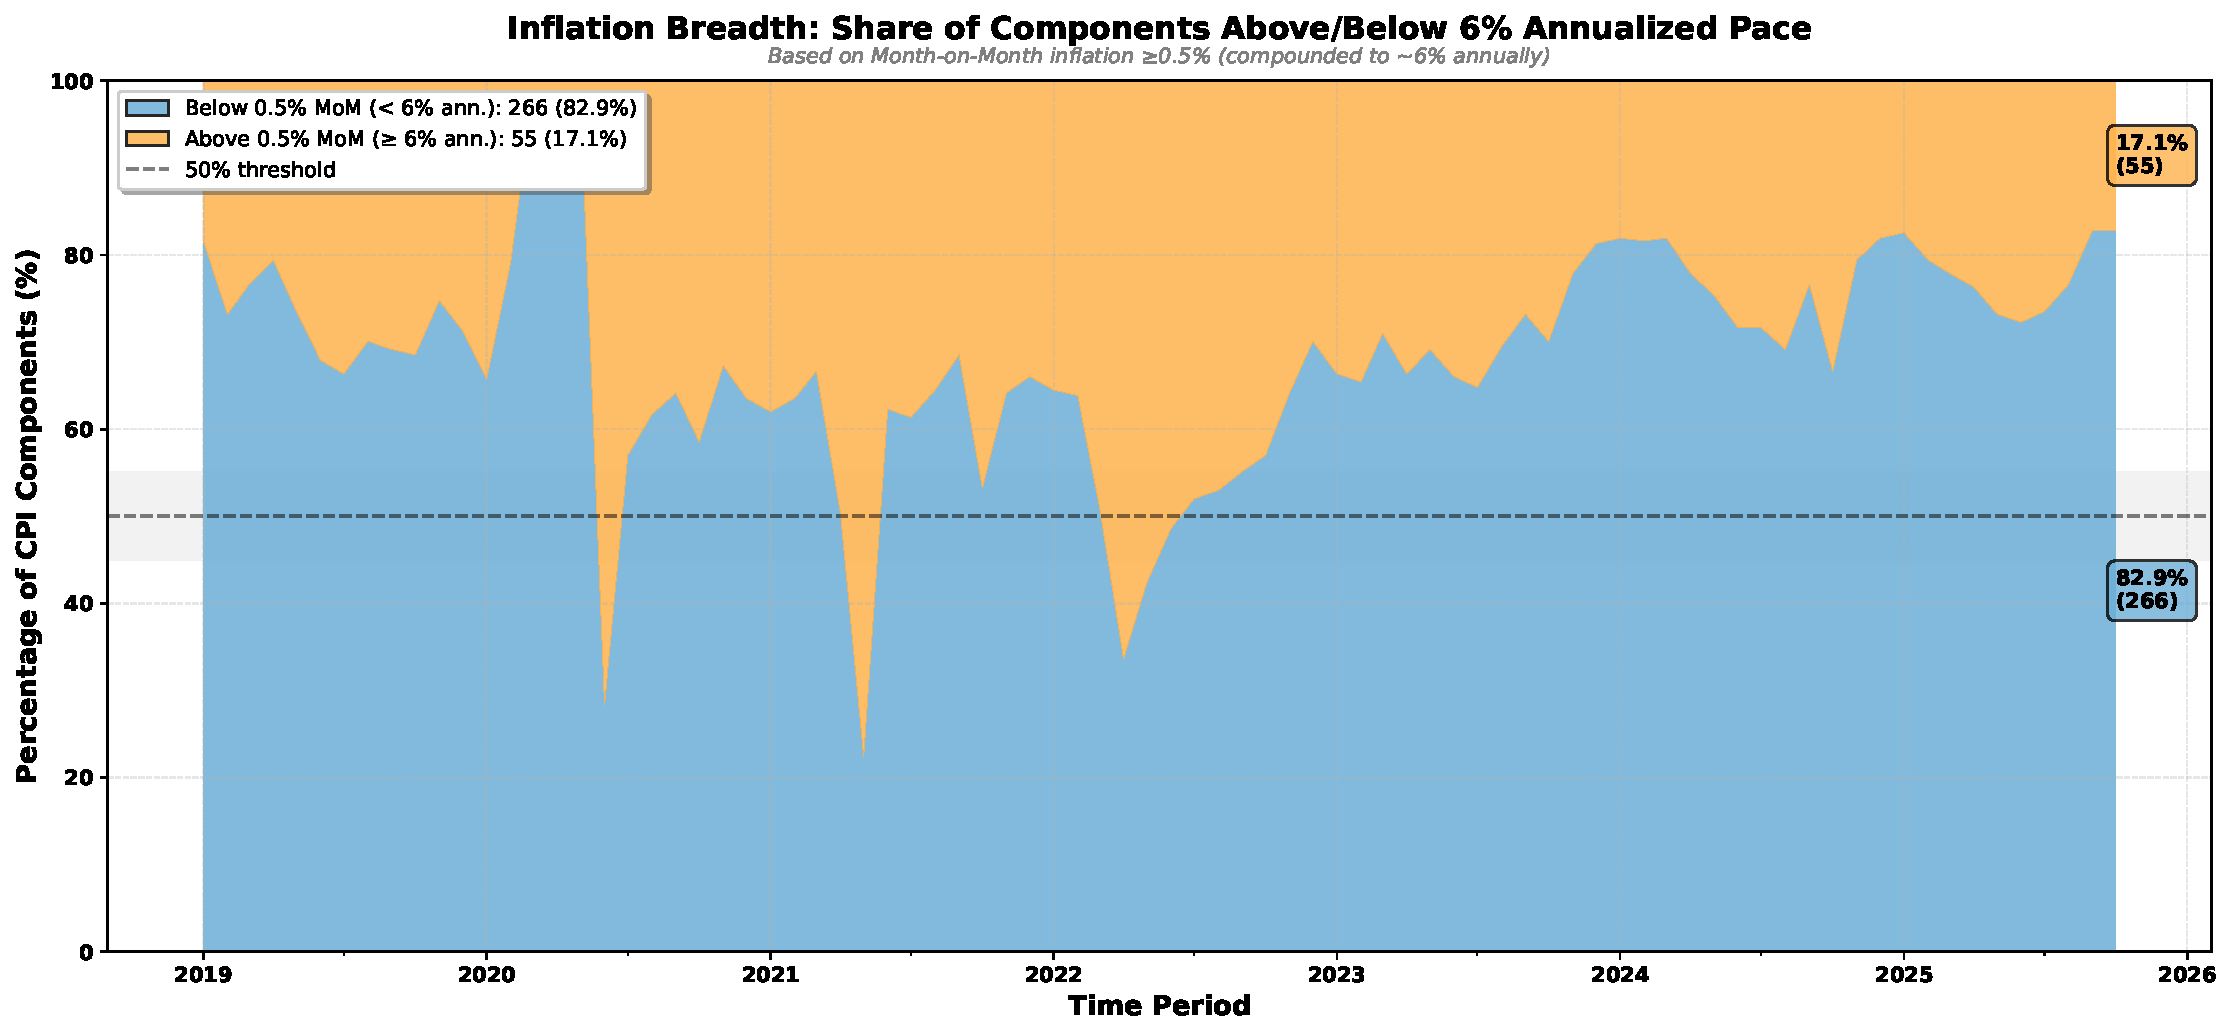
\includegraphics[keepaspectratio]{inflation_analysis_files/figure-pdf/fig-mom-threshold-6-output-1.pdf}}

}

\caption{\label{fig-mom-threshold-6}Inflation Breadth: Share of
Components Above/Below 6\% Annualized Pace}

\end{figure}%

\subsubsection{4\% Annualized Threshold (0.33\%
MoM)}\label{annualized-threshold-0.33-mom}

\begin{figure}[H]

\centering{

\pandocbounded{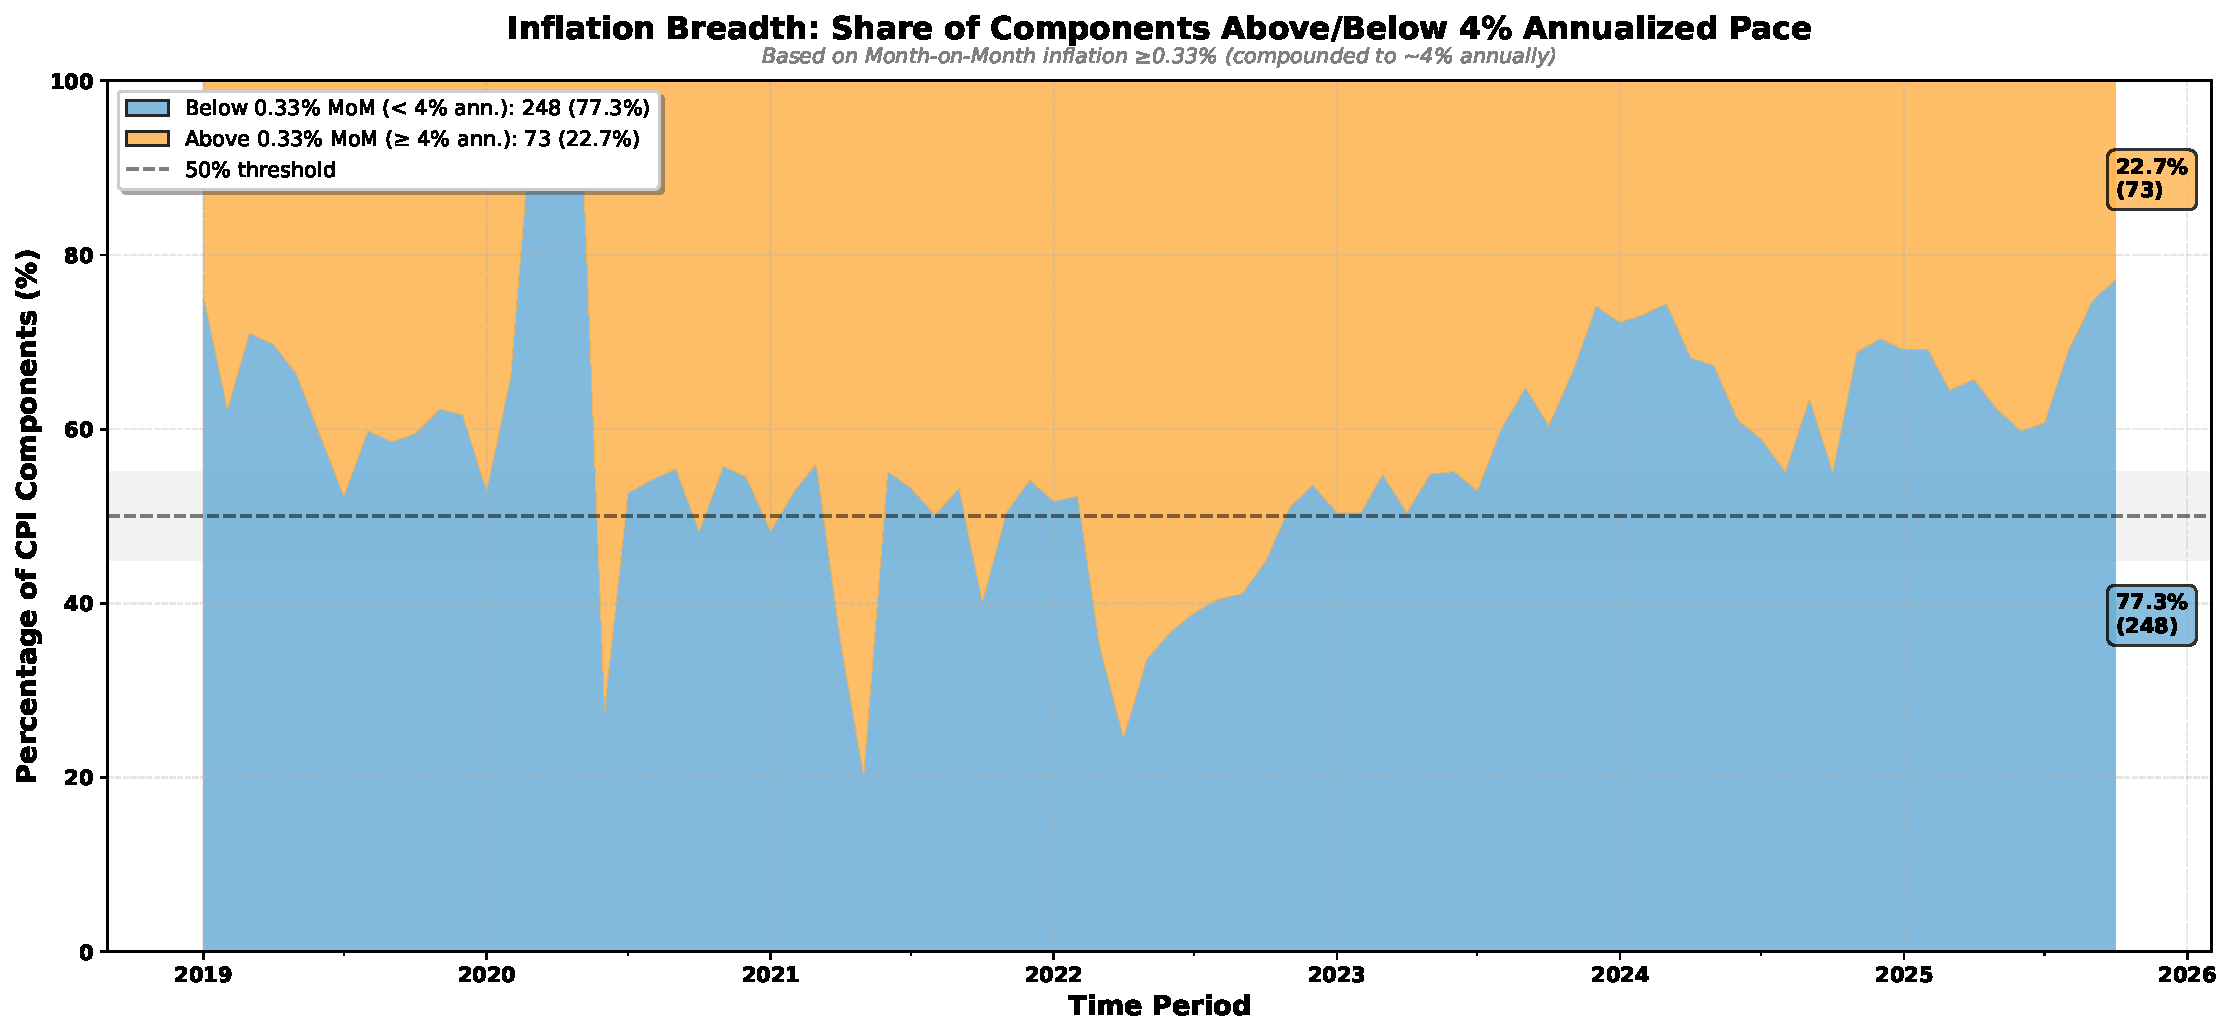
\includegraphics[keepaspectratio]{inflation_analysis_files/figure-pdf/fig-mom-threshold-4-output-1.pdf}}

}

\caption{\label{fig-mom-threshold-4}Inflation Breadth: Share of
Components Above/Below 4\% Annualized Pace}

\end{figure}%

\subsubsection{MoM Threshold Insights}\label{mom-threshold-insights}

\subsubsection{Current Month (October
2025)}\label{current-month-october-2025}

\paragraph{6\% Annualized Threshold}\label{annualized-threshold}

\begin{itemize}
\item
  \textbf{17.1\%} (55 components) are currently inflating above the 6\%
  annualized pace (\textgreater0.5\% MoM)
\item
  Inflation pressure is \textbf{concentrated in select items},
  suggesting \textbf{contained inflation} with most components cooling
\end{itemize}

\paragraph{4\% Annualized Threshold}\label{annualized-threshold-1}

\begin{itemize}
\item
  \textbf{22.7\%} (73 components) are inflating above the 4\% annualized
  pace (\textgreater0.33\% MoM)
\item
  The majority of components are \textbf{below the 4\% lower bound},
  potentially signaling room for \textbf{policy easing}
\end{itemize}

\paragraph{Change from Year Ago (October
2024)}\label{change-from-year-ago-october-2024}

\begin{itemize}
\item
  The share of components above 6\% annualized pace has
  \textbf{decreased by 16.2 percentage points}
\item
  The share of components above 4\% annualized pace has
  \textbf{decreased by 22.1 percentage points}
\end{itemize}

\paragraph{12-Month Trend}\label{month-trend}

\begin{itemize}
\item
  Components above 6\% threshold show \textbf{no clear trend} over the
  past year
\item
  Components above 4\% threshold show \textbf{no clear trend} over the
  past year
\end{itemize}

\subsection{Key Insights}\label{key-insights}

\subsubsection{Current Month (October
2025)}\label{current-month-october-2025-1}

\begin{itemize}
\item
  \textbf{11.2\%} of CPI components are within the RBI target band
  (4-6\%)
\item
  \textbf{12.8\%} of components are experiencing above-target inflation
  (\textgreater6\%)
\item
  \textbf{76.0\%} of components are below the 4\% threshold
\item
  The dominant category is \textbf{Moderate (2-4\%)} with
  \textbf{28.0\%} of all components
\end{itemize}

\subsubsection{Change from Year Ago (October
2024)}\label{change-from-year-ago-october-2024-1}

\begin{itemize}
\tightlist
\item
  Inflation distribution remains relatively \textbf{stable}
\end{itemize}

\section{Seasonality Analysis}\label{seasonality-analysis}

\subsection{CPI Ex Vegetables}\label{cpi-ex-vegetables}

\begin{figure}[H]

\centering{

\pandocbounded{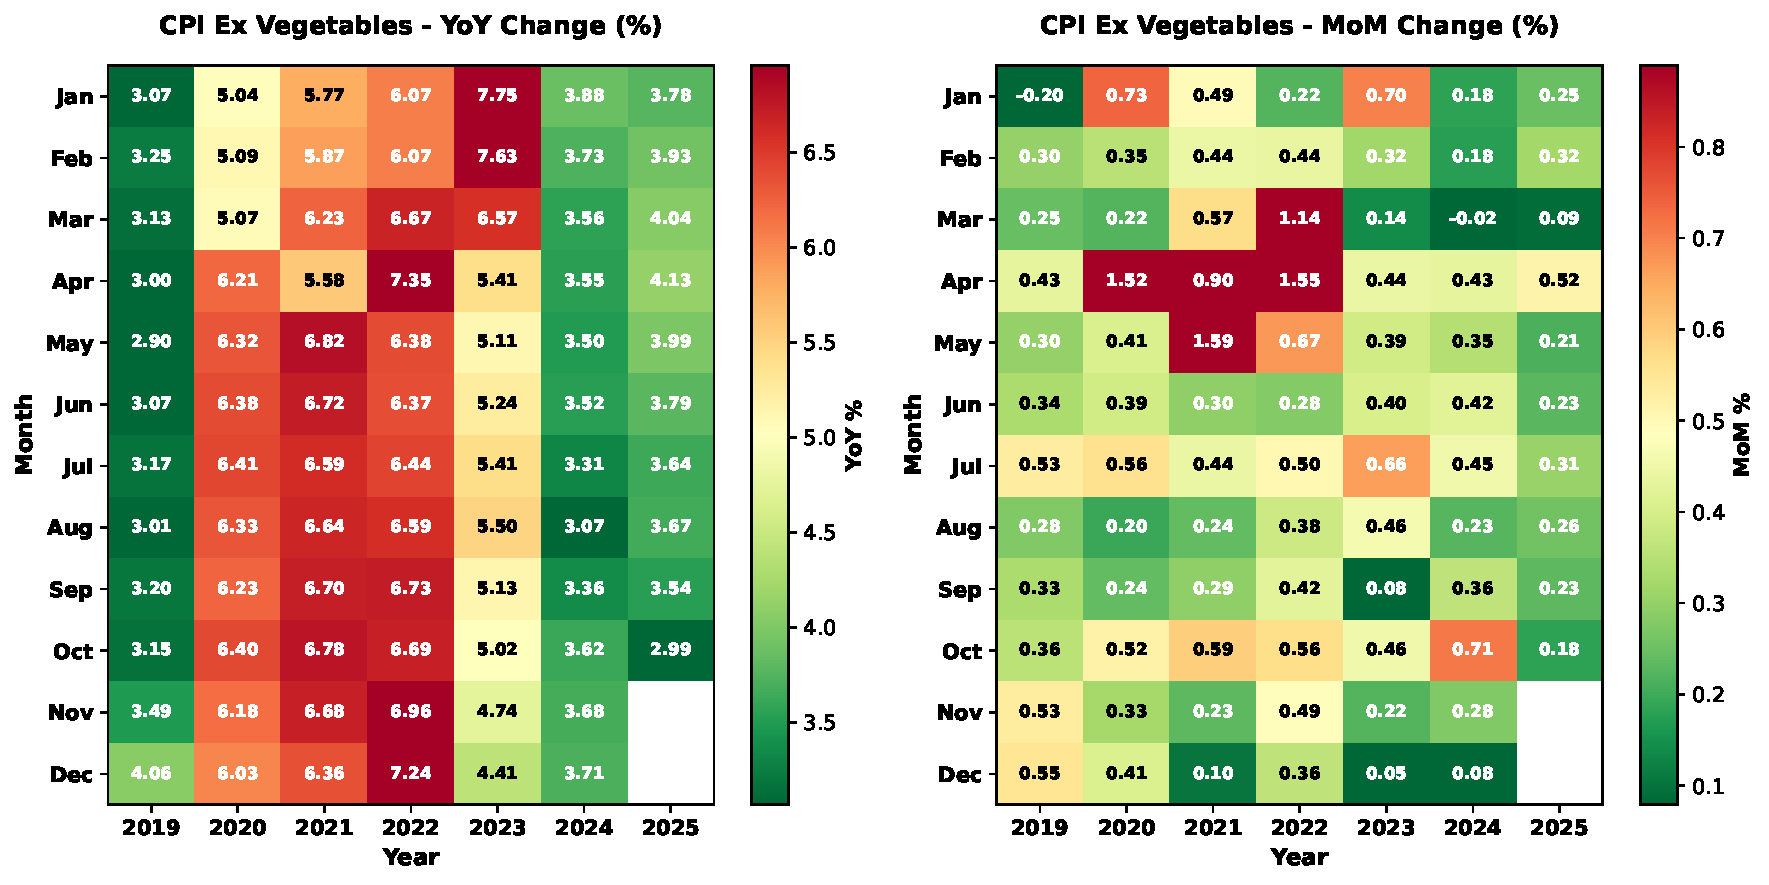
\includegraphics[keepaspectratio]{inflation_analysis_files/figure-pdf/fig-seasonality-exveggies-output-1.pdf}}

}

\caption{\label{fig-seasonality-exveggies}CPI Excluding Vegetables -
Seasonality Patterns (YoY and MoM)}

\end{figure}%

\subsection{Core CPI (Ex Food, Beverages \&
Fuel)}\label{core-cpi-ex-food-beverages-fuel}

\begin{figure}[H]

\centering{

\pandocbounded{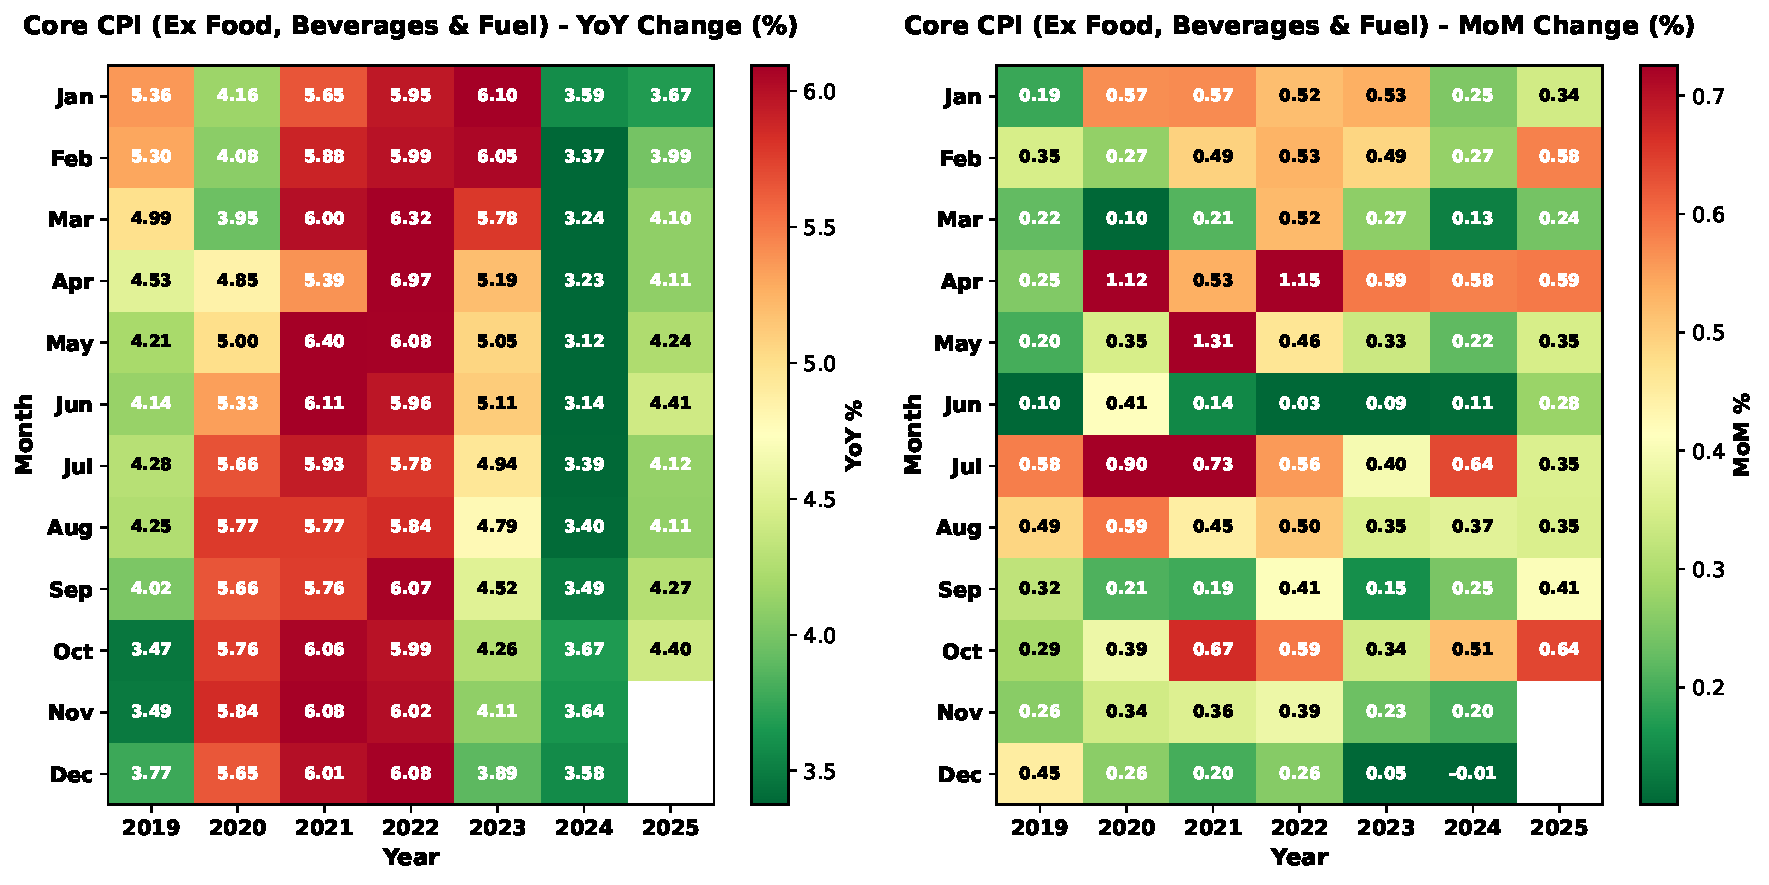
\includegraphics[keepaspectratio]{inflation_analysis_files/figure-pdf/fig-seasonality-core-output-1.pdf}}

}

\caption{\label{fig-seasonality-core}Core CPI (Excluding Food, Beverages
\& Fuel \& Light) - Seasonality Patterns (YoY and MoM)}

\end{figure}%

\subsection{Personal Care \& Effects}\label{personal-care-effects}

\begin{figure}[H]

\centering{

\pandocbounded{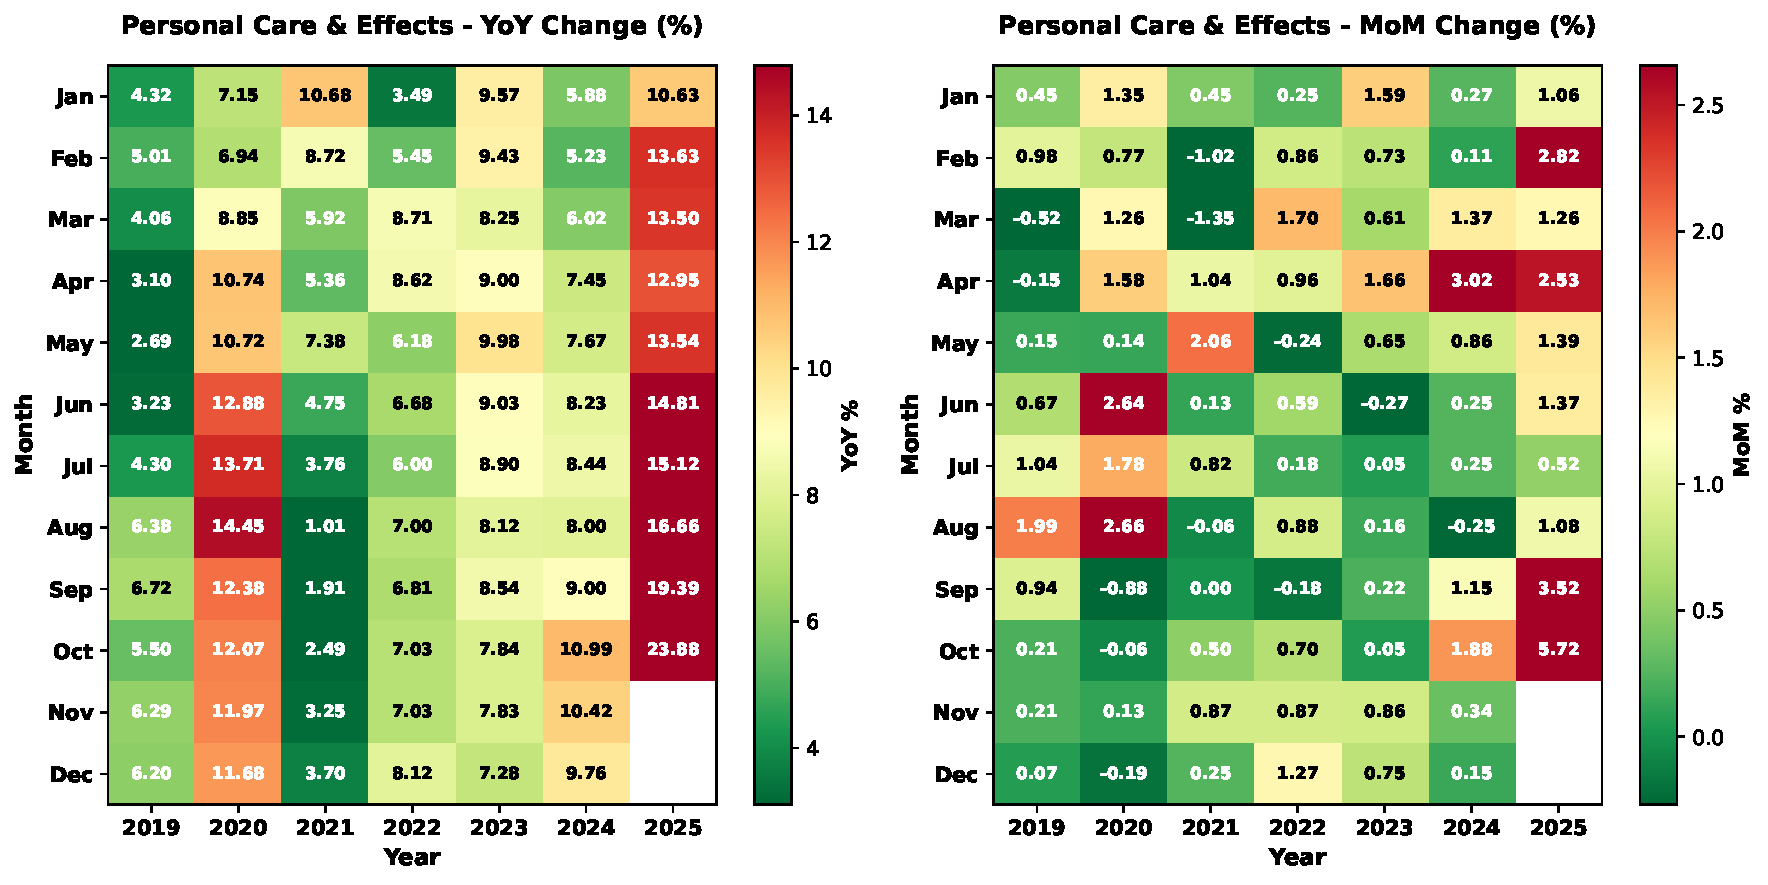
\includegraphics[keepaspectratio]{inflation_analysis_files/figure-pdf/fig-seasonality-personal-output-1.pdf}}

}

\caption{\label{fig-seasonality-personal}CPI Miscellaneous (Personal
Care \& Effects) - Seasonality Patterns (YoY and MoM)}

\end{figure}%

\subsection{Food Price Index}\label{food-price-index}

\begin{figure}[H]

\centering{

\pandocbounded{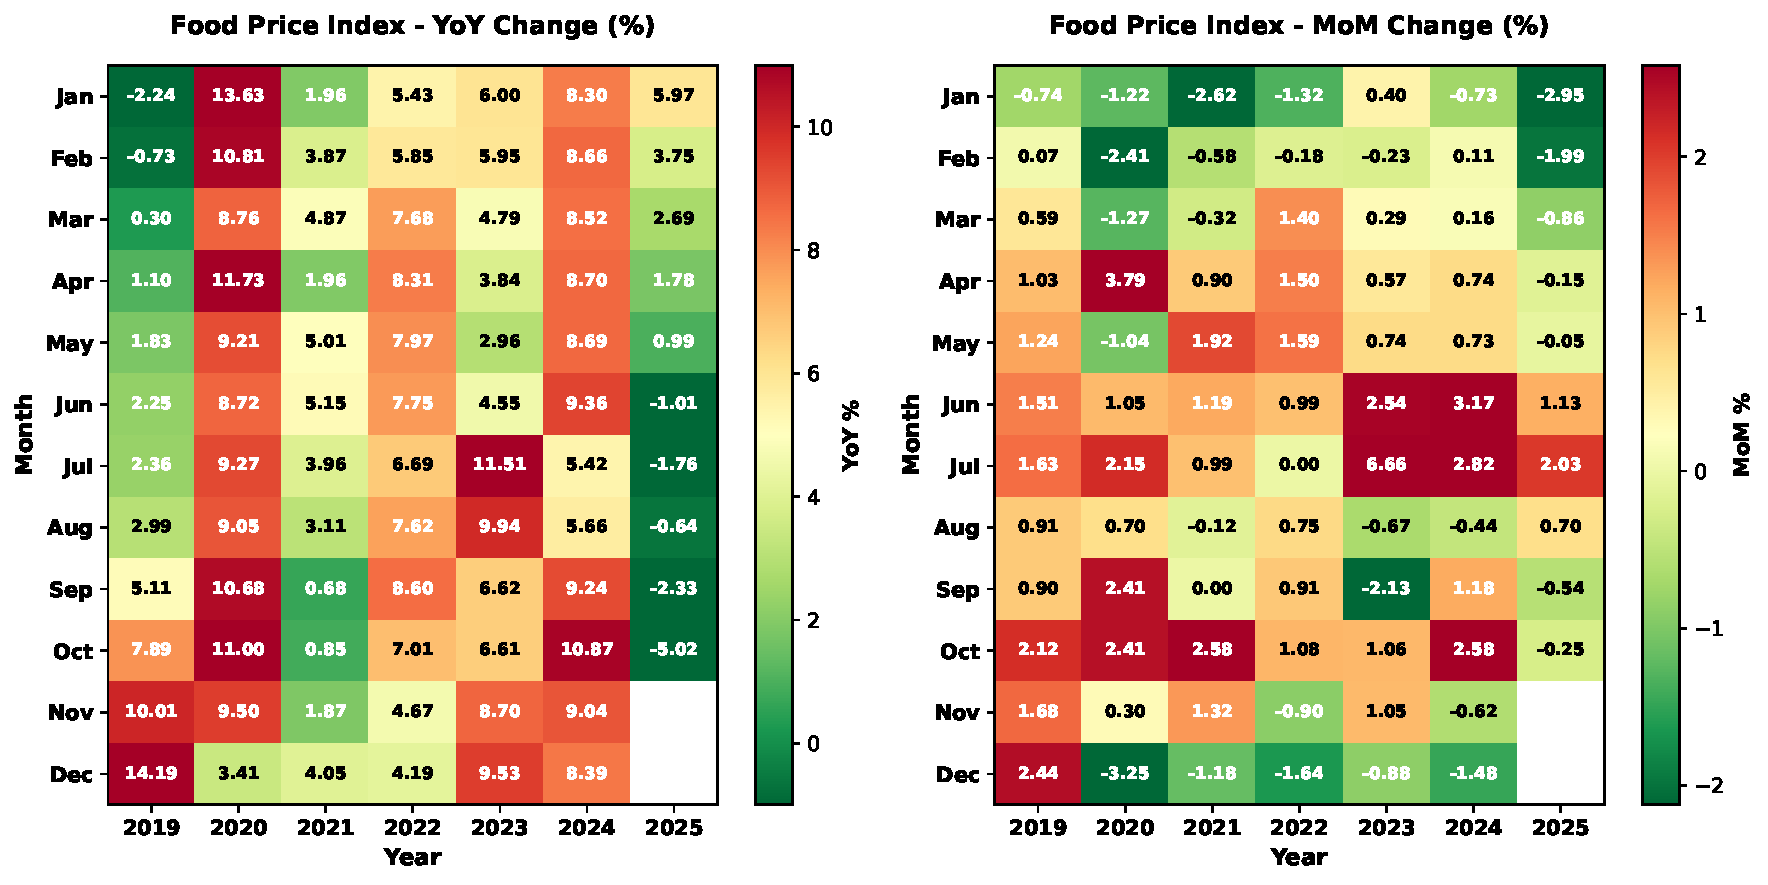
\includegraphics[keepaspectratio]{inflation_analysis_files/figure-pdf/fig-seasonality-food-output-1.pdf}}

}

\caption{\label{fig-seasonality-food}Consumer Food Price Index -
Seasonality Patterns (YoY and MoM)}

\end{figure}%

\subsection{CPI (Excluding Gold)}\label{cpi-excluding-gold}

!{[}Consumer Food Price Index (Excluding
Gold){]}(inflation\_analysis\_files/figure-pdf/fig-seasonality-cpi-(ex-gold-output-1.pdf)\{\#fig-seasonality-cpi-(ex-gold\}

\subsection{CPI (Excluding Gold and
Silver)}\label{cpi-excluding-gold-and-silver}

!{[}Consumer Food Price Index (Excluding Gol and
Silver){]}(inflation\_analysis\_files/figure-pdf/fig-seasonality-cpi-(ex-gold-and-silver-output-1.pdf)\{\#fig-seasonality-cpi-(ex-gold-and-silver\}

\section{Inflation Trends Over Time}\label{inflation-trends-over-time}

\subsection{Recent Trends (Last 7
Years)}\label{recent-trends-last-7-years}

\begin{figure}[H]

\centering{

\pandocbounded{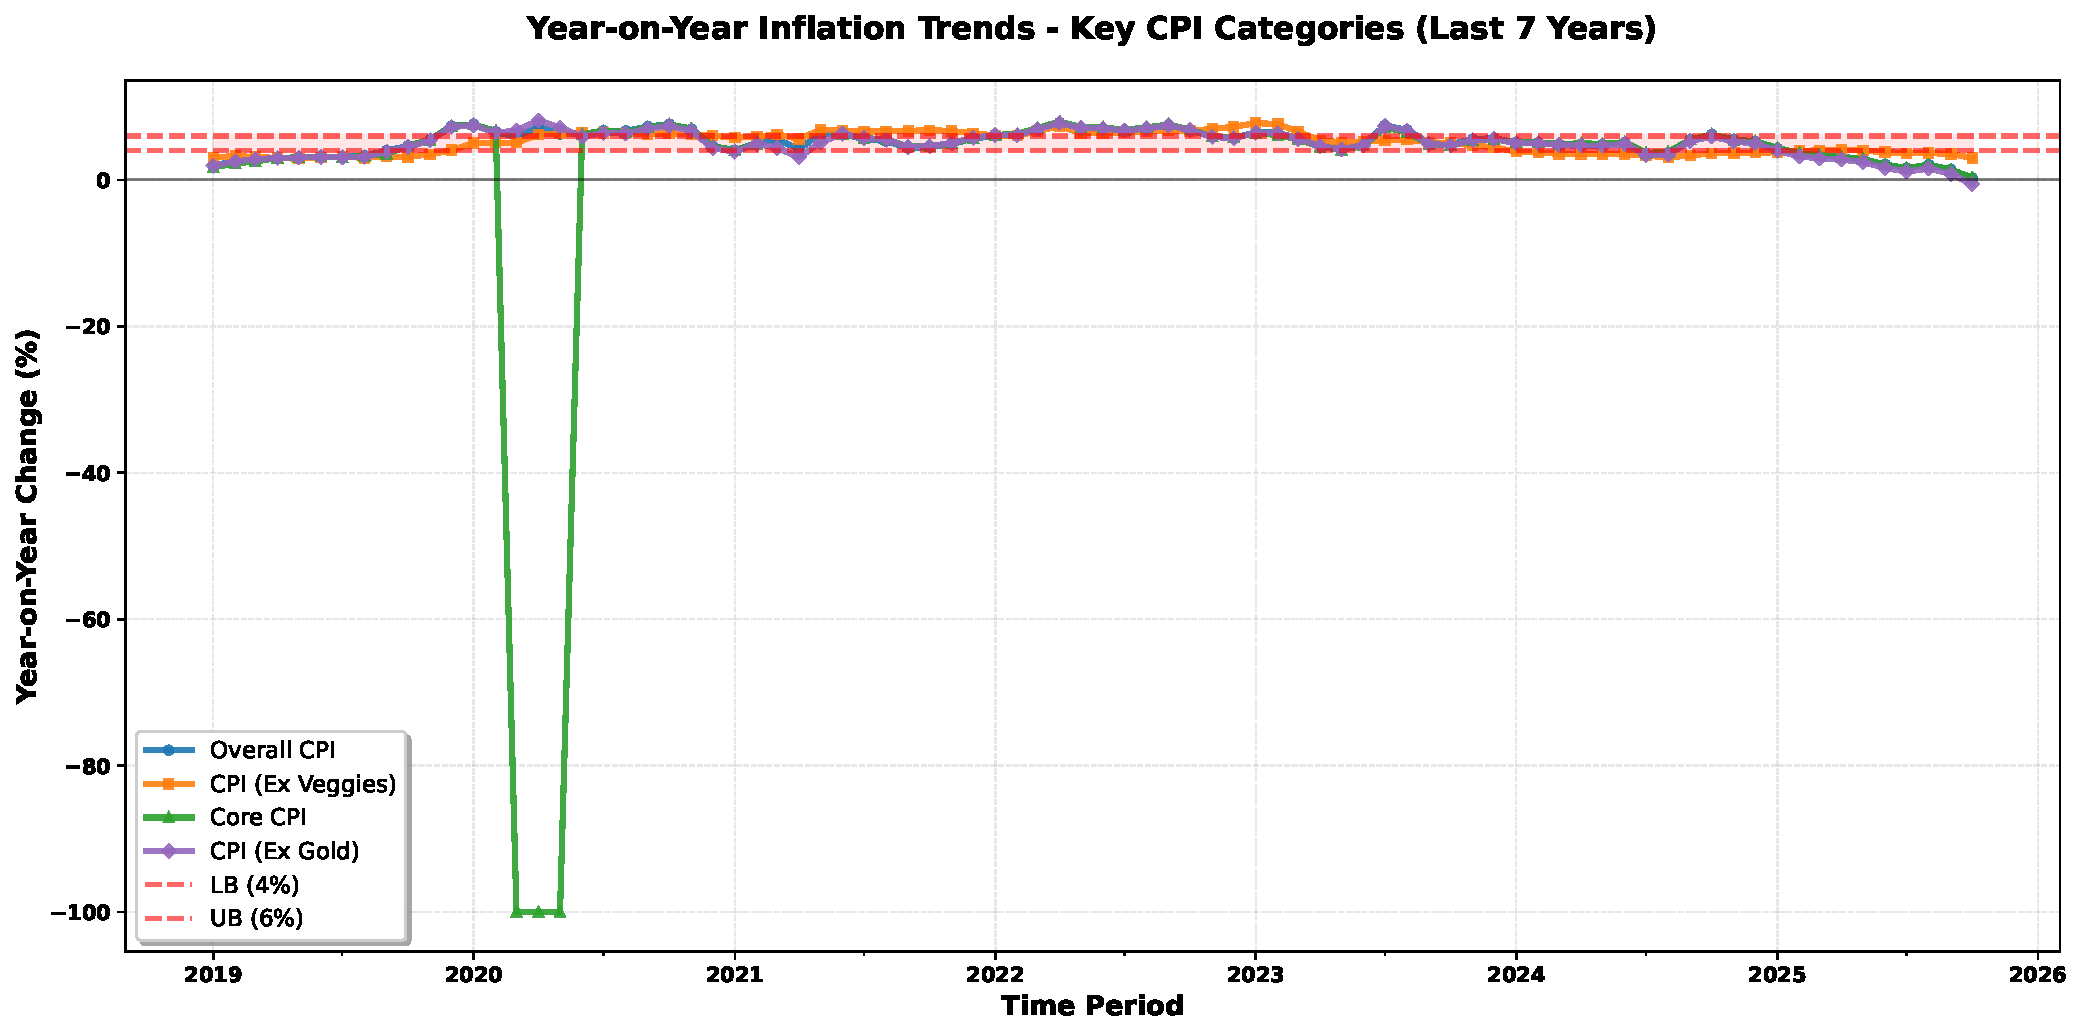
\includegraphics[keepaspectratio]{inflation_analysis_files/figure-pdf/fig-yoy-trends-output-1.pdf}}

}

\caption{\label{fig-yoy-trends}Year-on-Year Inflation Trends - CPI
Categories Comparison}

\end{figure}%

\subsection{Month on Month Trend}\label{month-on-month-trend}

\begin{figure}[H]

\centering{

\pandocbounded{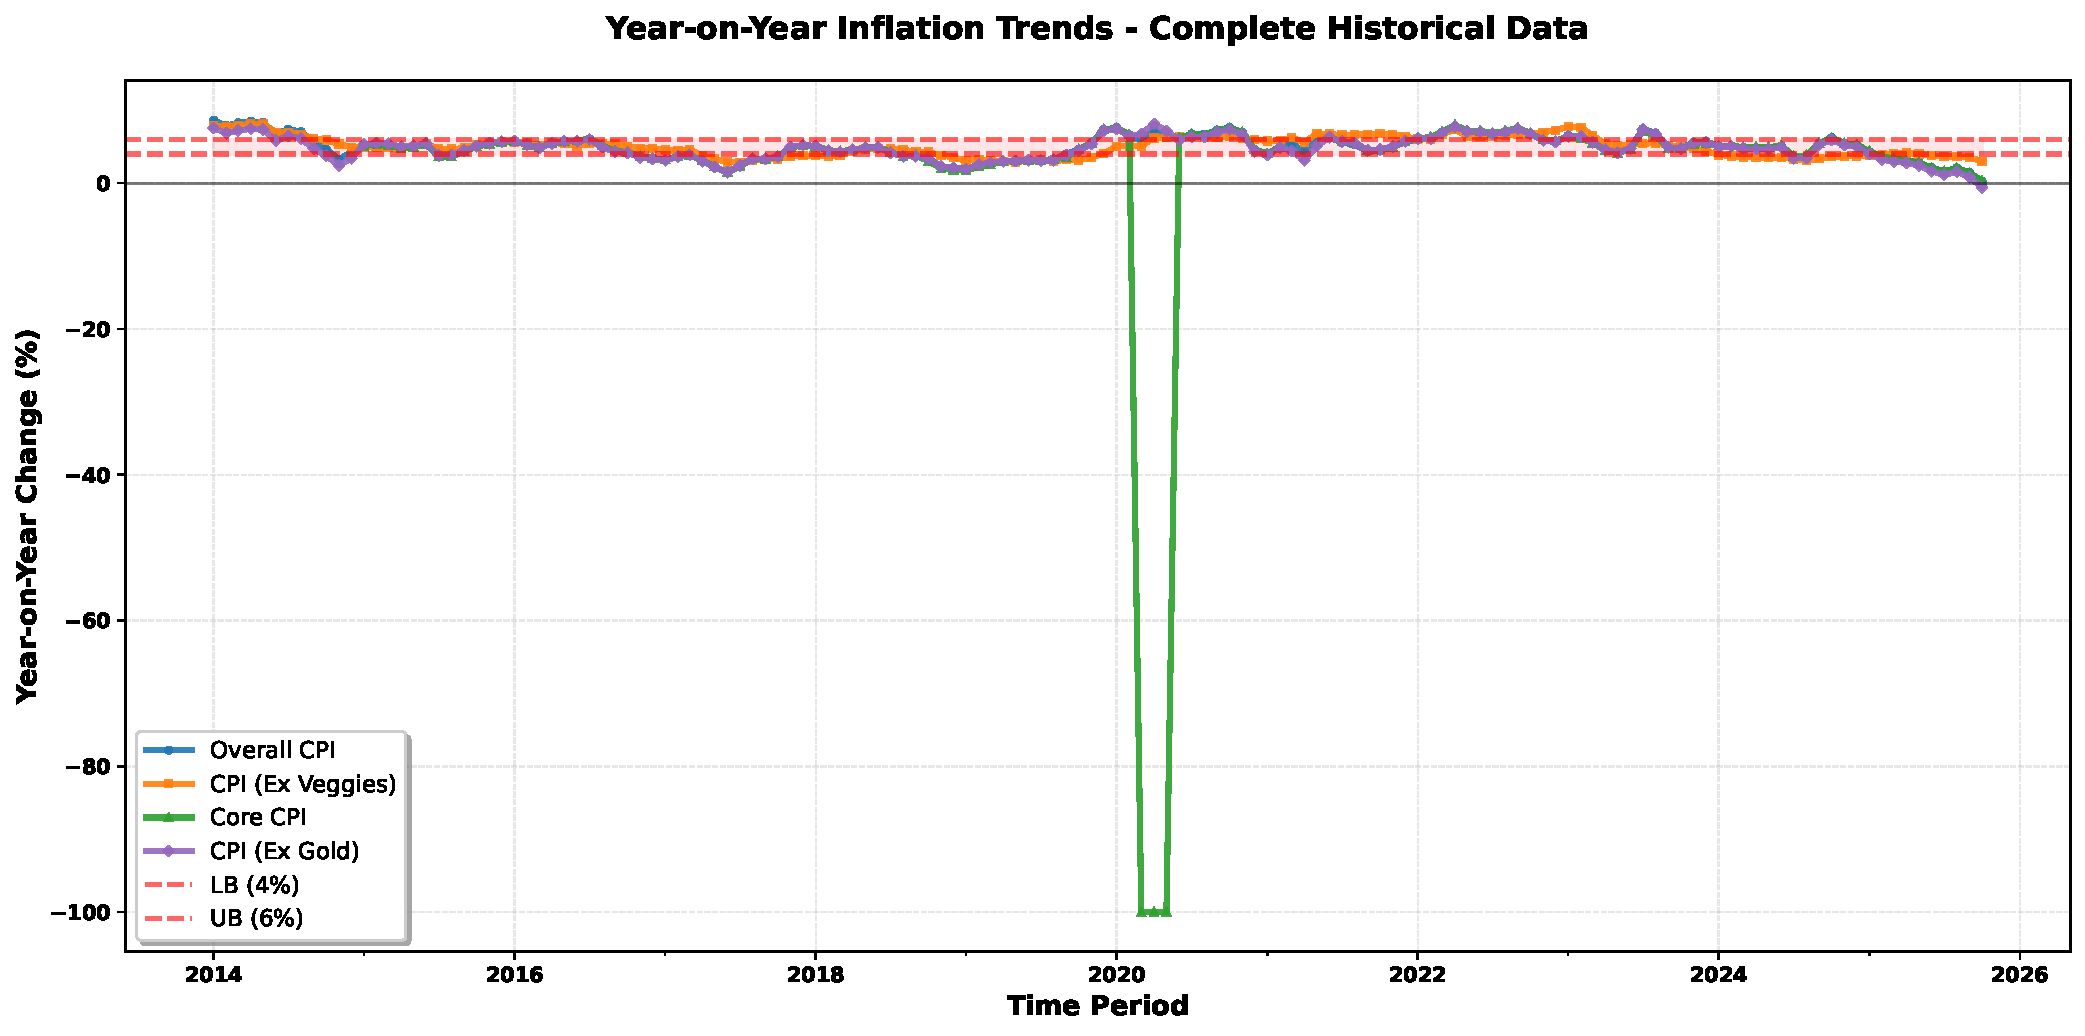
\includegraphics[keepaspectratio]{inflation_analysis_files/figure-pdf/fig-mom-trends-output-1.pdf}}

}

\caption{\label{fig-mom-trends}Month-on-Month Inflation Trends - CPI
Categories Comparison}

\end{figure}%

\subsection{Historical Overview}\label{historical-overview}

\begin{figure}[H]

\centering{

\pandocbounded{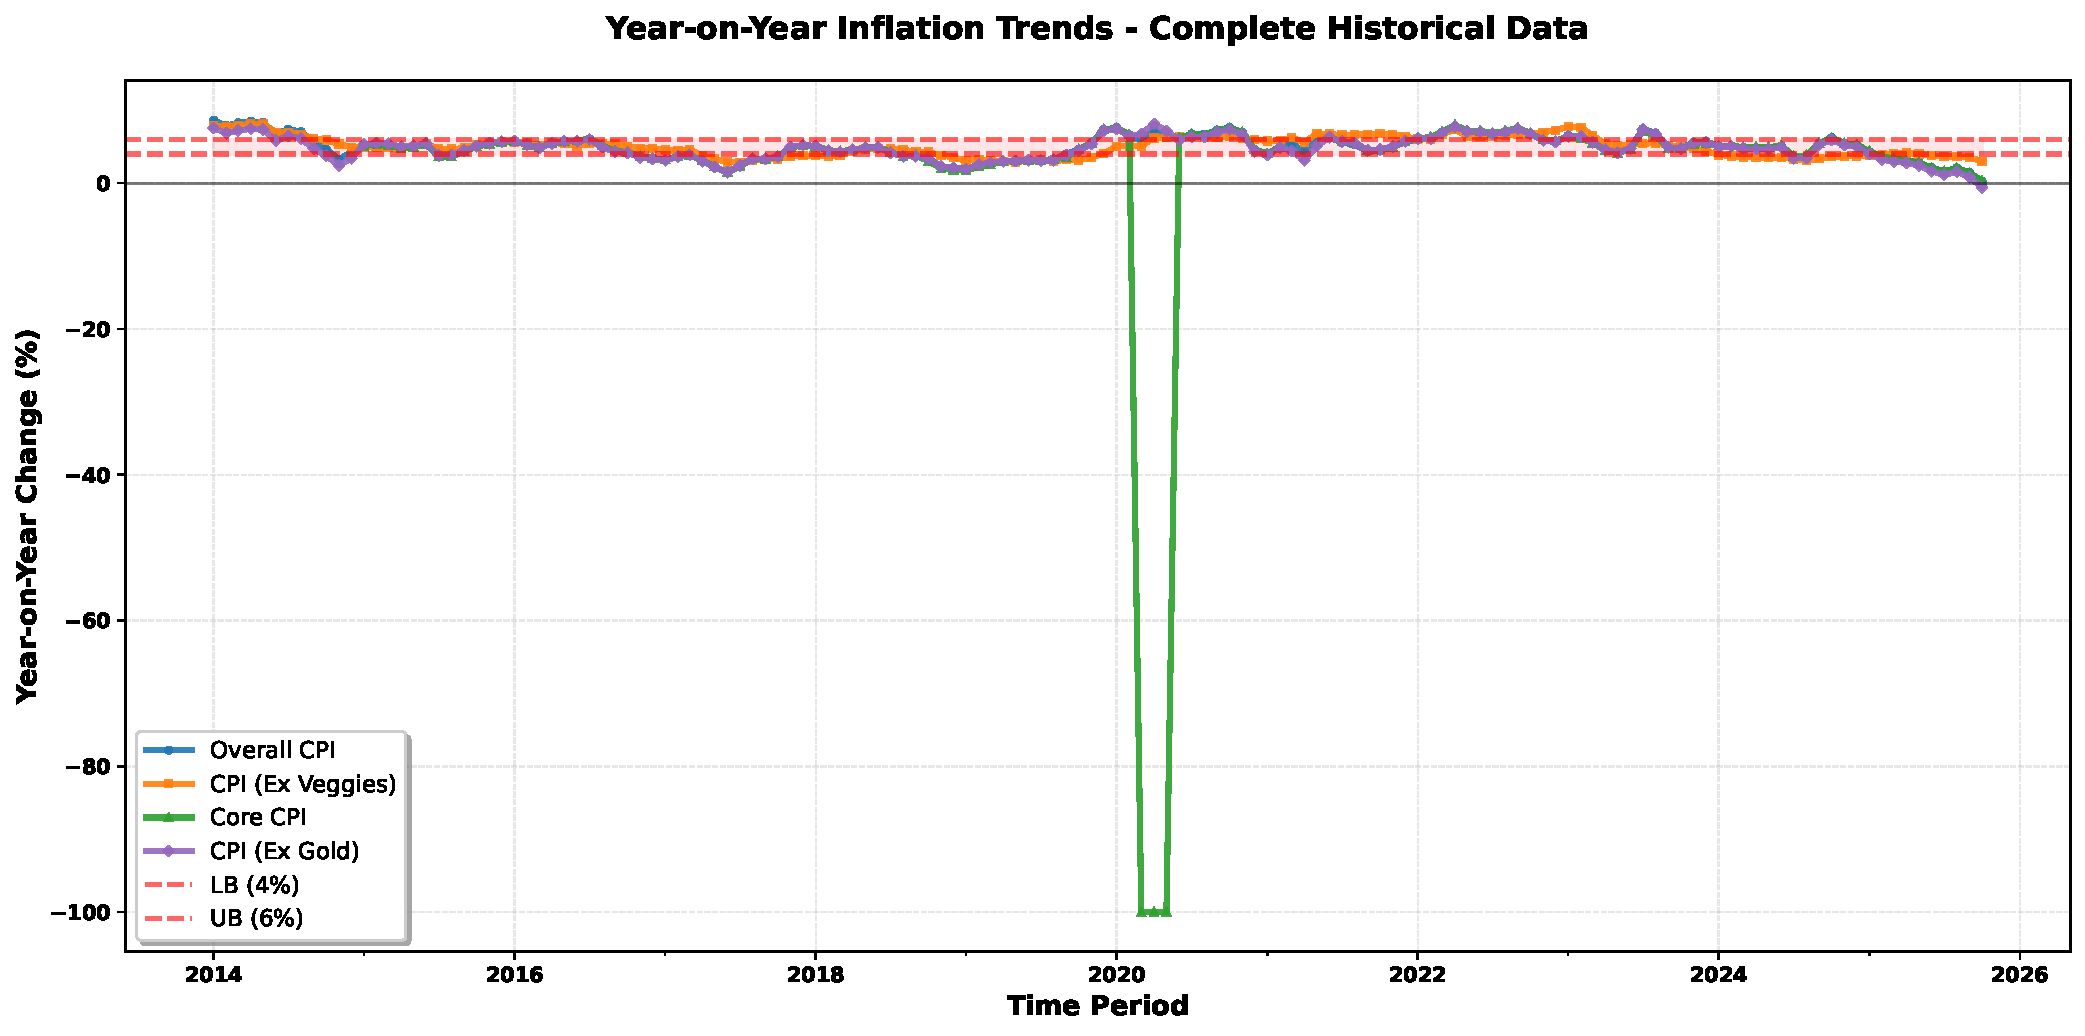
\includegraphics[keepaspectratio]{inflation_analysis_files/figure-pdf/fig-yoy-trends-full-output-1.pdf}}

}

\caption{\label{fig-yoy-trends-full}Year-on-Year Inflation Trends -
Complete Historical Data}

\end{figure}%




\end{document}
